% Modular manuscript. Use make source for a flat, single-TeX export.
% Official Springer Nature template package v3.1, December 2024.
\documentclass[pdflatex,sn-mathphys-ay]{sn-jnl}
\usepackage{graphicx}
\usepackage{amsmath,amssymb,amsthm}
\usepackage{booktabs,tabularx}
\usepackage[title]{appendix}
\providecommand{\tightlist}{\setlength{\itemsep}{0pt}\setlength{\parskip}{0pt}}
\DeclareUnicodeCharacter{03BB}{\ensuremath{\lambda}}
\DeclareUnicodeCharacter{03C4}{\ensuremath{\tau}}
\DeclareUnicodeCharacter{03B4}{\ensuremath{\delta}}
\DeclareUnicodeCharacter{03BC}{\ensuremath{\mu}}
\DeclareUnicodeCharacter{2265}{\ensuremath{\ge}}
\DeclareUnicodeCharacter{2264}{\ensuremath{\le}}
\DeclareUnicodeCharacter{2248}{\ensuremath{\approx}}
\DeclareUnicodeCharacter{2212}{\ensuremath{-}}
\DeclareUnicodeCharacter{221A}{\ensuremath{\surd}}
\theoremstyle{thmstyleone}
\newtheorem{theorem}{Theorem}[section]
\newtheorem{proposition}[theorem]{Proposition}
\newtheorem{lemma}[theorem]{Lemma}
\theoremstyle{thmstylethree}
\newtheorem{definition}{Definition}[section]
\newcommand{\DraftPlaceholder}[1]{\par\noindent\textit{Draft placeholder: #1}\par}
\hypersetup{pdftitle={Bartender: Continuous Worktree Reconciliation with Author-Routed Conflict Handback for Resident Multi-Agent Development},pdfauthor={}}
\raggedbottom

\begin{document}
\title[Bartender]{Bartender: Continuous Worktree Reconciliation with Author-Routed Conflict Handback for Resident Multi-Agent Development}
\author[1]{\fnm{Author} \sur{TBD}}
\affil[1]{\orgname{Affiliation TBD}}
\abstract{When several coding agents edit one codebase, current tools use one of two arrangements. A shared working copy keeps every agent on the same state but lets them overwrite each other. Per-agent Git worktrees isolate work but are merged only on demand, one worktree at a time, and discarded afterwards, so branches drift apart between merges. This paper describes Bartender, the synchronization mechanism of Kota, an open-source environment for resident coding agents---agents that persist in a workspace across tasks and sessions. Bartender keeps a persistent worktree for each agent and synchronizes all worktrees frequently: it integrates every worktree that applies cleanly onto the shared branch, holds the ones that conflict, and hands each conflict back to the agent that authored it, together with the current base and the failing commit. We state the mechanism's premises and give a mathematical account of why it is designed this way. A discrete-event simulation then tests the expected benefits of frequent synchronization, and of real-time conflict resolution by the owning agent, against on-demand synchronization and human review. In the simulation, in-place repair needs up to 2.8 times as many repairs and 12 times as much repair work as Bartender at high overlap, and repairing each conflict at once keeps virtually every conflict resolvable within the observation window, where a wait of four characteristic times leaves 48--73 percent unresolved.}
\keywords{multi-agent systems, software integration, version control, conflict repair}
\maketitle
\section{Introduction}\label{sec:introduction}

Multi-agent coding systems today edit files in one of two ways. In the first, all agents work in a shared working copy. Everyone sees the same state and nothing has to be merged, but agents overwrite each other's edits and a half-finished change is visible to everyone immediately. In the second, each agent gets its own Git worktree. Work is isolated, but the worktree is a temporary staging area for one task: it is merged only when someone orders a merge, the order covers that one worktree, and the worktree is discarded afterwards. Between orders, branches drift apart, and each agent works on a base that no longer matches the others'.

Merging one worktree at a time is a habit inherited from human teams, not a requirement of the problem. Humans cannot merge everyone's work at once because coordinating everyone at once is expensive. Resident agents---agents that live in the workspace across tasks and sessions, rather than being started for one task and discarded---do not have that constraint: they can be synchronized together, as often as one likes, without anyone's attention.

Bartender, the synchronization mechanism of Kota \citep{kota-source,wu2026kotalongtermteammates}, is built on that observation. It keeps the isolation of per-agent worktrees and recovers the unity of a shared copy by synchronizing all worktrees at high frequency. Each synchronization tries every worktree against the shared branch. Worktrees that apply cleanly are integrated at once. Worktrees that conflict are held, and the conflict is handed back to the agent that authored the work, with the current base and the failing commit, so that the author repairs it against the latest state instead of a coordinator guessing at intent. Worktrees are not discarded: each one belongs to its agent for as long as the agent exists, survives the agent sleeping or changing sessions, and is removed only when the agent is permanently dismissed. The trade-off is that merging a single worktree on command is no longer the normal mode of operation; a user can still instruct one agent to synchronize its own tree. In exchange, all agents stay on one state and never edit the same copy.

The paper makes two claims about this design. First, synchronization should be frequent and cover all worktrees. Two edits can conflict only if they were made concurrently, that is, with no synchronization between them: an edit made after a synchronization starts from a base that already contains the earlier edit, so the two are sequential, not concurrent. Synchronization turns concurrency into sequence, and the synchronization interval is the width of the concurrency window. Second, a conflict should be repaired immediately by the agent that owns the conflicting work, not queued for human review. While a conflict waits, the context its repair must reconcile keeps growing, and a repair that waits long enough is overtaken by new work and has to be redone.

Bartender was built after experiencing long-lived branches and large rebases in tools that merge on demand. In the environment where it now runs, conflicts have been rare; Section~\ref{sec:deployment} reports what the retained records show.

The contributions are three. First, a clearly specified, reusable mechanism for continuous reconciliation of resident agents' worktrees with author-routed handback of conflicts. Second, an analysis of its properties under explicit assumptions: proofs where they exist, first-order scaling laws where they do not, and the boundary of the model. Third, an account of the shipped implementation, and a deployment record. The contribution is the combination and its stated guarantees, not any single component.

The rest of the paper follows the mechanism from problem to limits. Section~\ref{sec:related-work} positions Bartender against merge queues, incremental integration, and agent systems for concurrent shared-state work. Section~\ref{sec:problem} defines the objects the analysis counts. Section~\ref{sec:mechanism} describes the mechanism as shipped, step by step. Section~\ref{sec:performance} gives the performance analysis. Section~\ref{sec:verification} verifies the implementation against the specification and tests the analysis in a synthetic model. Section~\ref{sec:deployment} reports the deployment record. Section~\ref{sec:discussion} discusses design choices, in particular why conflicts go back to the author rather than to a dedicated merge agent, and what the mechanism does not solve.
\section{Related work}\label{sec:related-work}

\textbf{Engineering practice.} Git worktrees give one repository several working directories, each on its own branch; they are the isolation primitive Bartender builds on and not a contribution of this paper \citep{git-worktree}. Merge queues and merge trains, as offered by GitHub and GitLab, serialize the integration of approved changes onto a protected branch, test each candidate against the branch state it will actually land on, and eject a candidate that fails \citep{github-merge-queue,gitlab-merge-trains}. Continuous integration in the sense of Fowler \citep{fowler-continuous-integration} and trunk-based development argue for integrating small changes often; Bartender applies the same argument to agents, whose integration cadence can be far higher than a human team's.

\textbf{Merge queues and Bartender.} A merge queue and Bartender differ not in how long a conflicting change waits---that depends on the author, not the mechanism---but in who closes the repair loop. A merge queue ejects the conflicting change and waits for the author to notice, repair, and re-enter it. Bartender dispatches the conflict to the authoring agent immediately, with the base and the failing commit, because the author is a resident agent that can be woken. When the queue's author-response delay is zero and the resolver is the owning agent, the two mechanisms coincide. In that sense Bartender completes the merge-queue design for resident agents rather than competing with it; Section~\ref{sec:performance} and Section~\ref{sec:verification} quantify what the missing loop costs when the author is a person, or an agent that nobody wakes.

\textbf{Agent systems for concurrent shared-state work.} Three recent systems address the same problem from different sides. Geng and Neubig \citep{geng2026-asynchronous} describe asynchronous software-engineering agents in which a manager creates an isolated worktree for each engineer, attempts to merge that engineer's branch into the main branch when a commit is submitted, and assigns any merge conflict to the engineer that produced the conflicting commit; the worktree is deleted after that engineer completes all assigned tasks or reaches its iteration limit. Liu et al.~\citep{liu2026-state-management} instead place agents in one shared workspace and mediate file operations: a write is accepted only while the target and the writer's read dependencies remain at the versions the writer observed; otherwise the write is rejected with current-state information so the agent can re-plan and retry. CoAgent \citep{lyu2026-coagent} fixes a serialization order at launch, serves order-filtered reads, notifies an affected reader when an earlier-ranked write may invalidate its premise so the reader can patch only the affected operations, and uses registered inverses to undo and reapply reversible writes that arrive out of order. GitHub's and GitLab's integration checks validate a candidate against the current branch before it lands \citep{github-merge-queue,gitlab-merge-trains}. None of the individual components---per-agent worktrees, checking before integration, handing a conflict back to its author---is new. Bartender differs in the arrangement: repeated, workspace-wide integration over per-agent worktrees that persist for the life of the agent, triggered when the workspace is idle and on request; clean commits land first, unchanged failures are retried mechanically after progress, and unresolved conflicts go to their authors. It does not provide write-time validation in a shared workspace \citep{liu2026-state-management} or serialization with filtered reads and undo \citep{lyu2026-coagent}. What this paper adds is the specification and analysis of that arrangement, not any individual primitive.

\textbf{Automatic conflict resolution.} MergeBERT \citep{svyatkovskiy2022-transformers} and DeepMerge \citep{dinella2023-deepmerge} resolve textual merge conflicts with learned models, without access to the intent of either author. They mark one end of a spectrum: resolution by a party that has neither author's context. Bartender's routing marks the other end: resolution by the party that has the most context about one side. Section~\ref{sec:discussion} uses this contrast to argue for author routing over a dedicated merge agent.

\textbf{Conflicts in human teams.} Studies of branch lifetime, merge conflict frequency, and the gap between textual and semantic conflicts in human teams \citep{bird2011-ownership,brun2011-conflicts} are background for this paper. We do not compare their conflict rates with ours: the denominators, team structures, and integration cadences differ too much for the numbers to be comparable.

Table~\ref{tab:integration-arrangements} summarizes the three integration arrangements the paper compares.

\begin{table}[tbp]
\caption{Three integration arrangements.}\label{tab:integration-arrangements}
\centering\small
\setlength{\tabcolsep}{4pt}
\renewcommand{\arraystretch}{1.12}
\begin{tabularx}{\textwidth}{@{}>{\raggedright\arraybackslash}p{0.18\textwidth}*{3}{>{\raggedright\arraybackslash}X}@{}}
\toprule
 & On-demand single-worktree merging & Merge queue / merge train \citep{github-merge-queue,gitlab-merge-trains} & Bartender \\
\midrule
Isolation unit & one worktree per task, discarded after the merge & branch or pull request & persistent worktree per agent \\
\addlinespace[3pt]
Synchronization trigger & a user or agent orders a merge of one worktree & entry into the queue & idle-triggered, or on an agent's or user's request; all worktrees \\
\addlinespace[3pt]
Recheck after a failure & none until the next order & candidates re-tested against the branch they will land on & failed worktrees retried after any pass that made progress \\
\addlinespace[3pt]
Who receives a conflict & whoever ordered the merge & the author, passively: the candidate is ejected & the authoring agent, actively dispatched with base and failing commit \\
\addlinespace[3pt]
Verification before landing & whatever the order runs & continuous-integration checks on the candidate & none; textual application only \\
\addlinespace[3pt]
Failure exit & conflict left to the orderer & ejection; the author re-enters the queue & first conflict handed back; the round ends \\
\bottomrule
\end{tabularx}
\end{table}
\section{Problem definition}\label{sec:problem}

\textbf{Objects.} A \emph{shared branch} is the branch that holds the integrated state of the project. Each agent owns one \emph{worktree} checked out on its own branch. The \emph{pending commits} of a worktree are the commits on its branch that are not yet on the shared branch. The \emph{base} of a synchronization attempt is the shared branch's head at the moment the attempt is made. A \emph{synchronization round} is one invocation of the mechanism over all worktrees.

\textbf{Four things that are easy to conflate.} A failed Git application is one cherry-pick that did not apply cleanly. A \emph{conflict event} is a failed application that the mechanism could not resolve mechanically and therefore hands to an agent. A \emph{retry} is a further attempt at the same commit after the base has advanced; several retries may belong to one conflict event. Finally, a small residue of cases needs a human decision because no automatic policy can decide them. The analysis and the deployment record count these separately.

\textbf{Three distinctions.} A merge that applies textually is not thereby correct; an agent can repair a conflict that Git could not, but that is not the same as a person having reviewed it; and an agent session's boundary is not a sensible synchronization period. Branch drift can be described by commits behind the shared branch, by changed lines, or by elapsed time, but each is a state indicator, not a conflict count and not a measure of user experience.

\textbf{Counting conventions.} In the shipped implementation, ``publishing'' a commit means cherry-picking it onto the shared branch of the local source repository; pushing the shared branch to a remote is a separate path and not part of the mechanism analyzed here. The unit of integration is the commit: a worktree with several pending commits is integrated commit by commit, and a prefix that applies cleanly stays integrated even if a later commit fails. Whenever Section~\ref{sec:performance} compares operation counts, the unit---worktree attempts, commit applications, or the mechanism's own snapshot and refresh operations---is declared before the comparison.
\section{Mechanism}\label{sec:mechanism}

\textbf{Architectural premise.} By default an agent edits only its own worktree. The rule is enforced by the agent's working directory and its instructions, not by a sandbox, and this is deliberate: a user can instruct an agent to read another agent's worktree, copy part of it, or merge selected changes without a full synchronization. Worktrees persist with their agents: a worktree is created when its agent is created, survives the agent sleeping or changing sessions, and is removed only when the agent is permanently dismissed. The analysis in Section~\ref{sec:performance} assumes the default: writes land only in the writer's own worktree.

The description below is of the implementation as shipped, at a pinned public commit of the Kota repository (\texttt{b3db3c82}), established by static reading of the source \citep{kota-source}. It is one synchronization round.

A round starts on one of three triggers. The optional automatic trigger polls every fifteen seconds and starts a round only when changes are pending, no agent in the workspace is observed working, no busy or conflict blocker is set, and three minutes have passed since both the last user prompt and the last completed synchronization; explicit requests by a user or by an agent enter the same synchronizer without that gate. The triggers are not this paper's subject; Section~\ref{sec:performance} treats the interval between rounds as a parameter.

\begin{enumerate}
\def\labelenumi{\arabic{enumi}.}
\item
  \textbf{Collect.} The mechanism lists the agents marked active whose worktrees exist, snapshots any uncommitted changes in the source repository and in each worktree, and enumerates each worktree's pending commits relative to the current base. Collection itself does not ask whether an agent is busy; that question belongs to the trigger, and the automatic trigger starts only when no agent is observed working. Neither guarantees that external writes have stopped.
\item
  \textbf{Attempt integration.} Worktrees are processed in a fixed order. For each worktree, pending commits are cherry-picked onto the shared branch one at a time. There is no separate candidate working area and no test or lint gate. A commit that applies cleanly is integrated; a commit that fails is aborted, recorded as a conflict for that agent, and the worktree is set aside for this pass while the remaining worktrees are processed. A commit that is empty against the current base---because an identical change already landed---is skipped. If a worktree's second commit fails, its first commit stays integrated: ``a failed integration exposes no half-finished state'' holds at the granularity of a commit, not of a worktree.
\item
  \textbf{Recheck.} After a full pass, the worktrees that failed are retried only if the pass integrated at least one commit, counting successful prefixes of failed worktrees as progress. Pending commits are recomputed against the new base on every attempt; there is no frozen pool. A pass that integrates nothing ends the round.
\item
  \textbf{Hand back.} When the round ends with unresolved conflicts, the mechanism sends one message, to the author of the first unresolved conflict. The message carries the shared branch's head as re-read at dispatch time, the failing commit, the raw Git error, and instructions: rebase the branch onto the given head, resolve the conflict, leave the worktree clean, and trigger synchronization again; if the intent cannot be preserved safely, ask for a product decision; never edit the source worktree. It does not carry the patch itself, a structured conflict location, or any semantic verification. Other unresolved conflicts are reported by count only in this round. Messages are de-duplicated by author, failing commit, and dispatch-time head.
\item
  \textbf{Finish or leave unresolved.} If the round ends with no unresolved conflicts, every active worktree is refreshed to the new base. If conflicts remain, the mechanism returns the conflict list and does not wait for any repair; the repair loop closes when the author, having repaired, triggers the next round. The command-line entry point waits up to thirty minutes for the dispatch result; that bound is on delivery of the message, not on the repair.
\end{enumerate}

Figure~\ref{fig:sync-loop} shows the round as a loop. The figure is taken from the Kota whitepaper \citep{wu2026kotalongtermteammates}, which describes the environment the mechanism belongs to; it draws the repair as returning into the loop, whereas the shipped implementation ends the round after dispatching the first unresolved conflict and re-enters the loop when the author triggers the next round.

\begin{figure}[tbp]
\centering
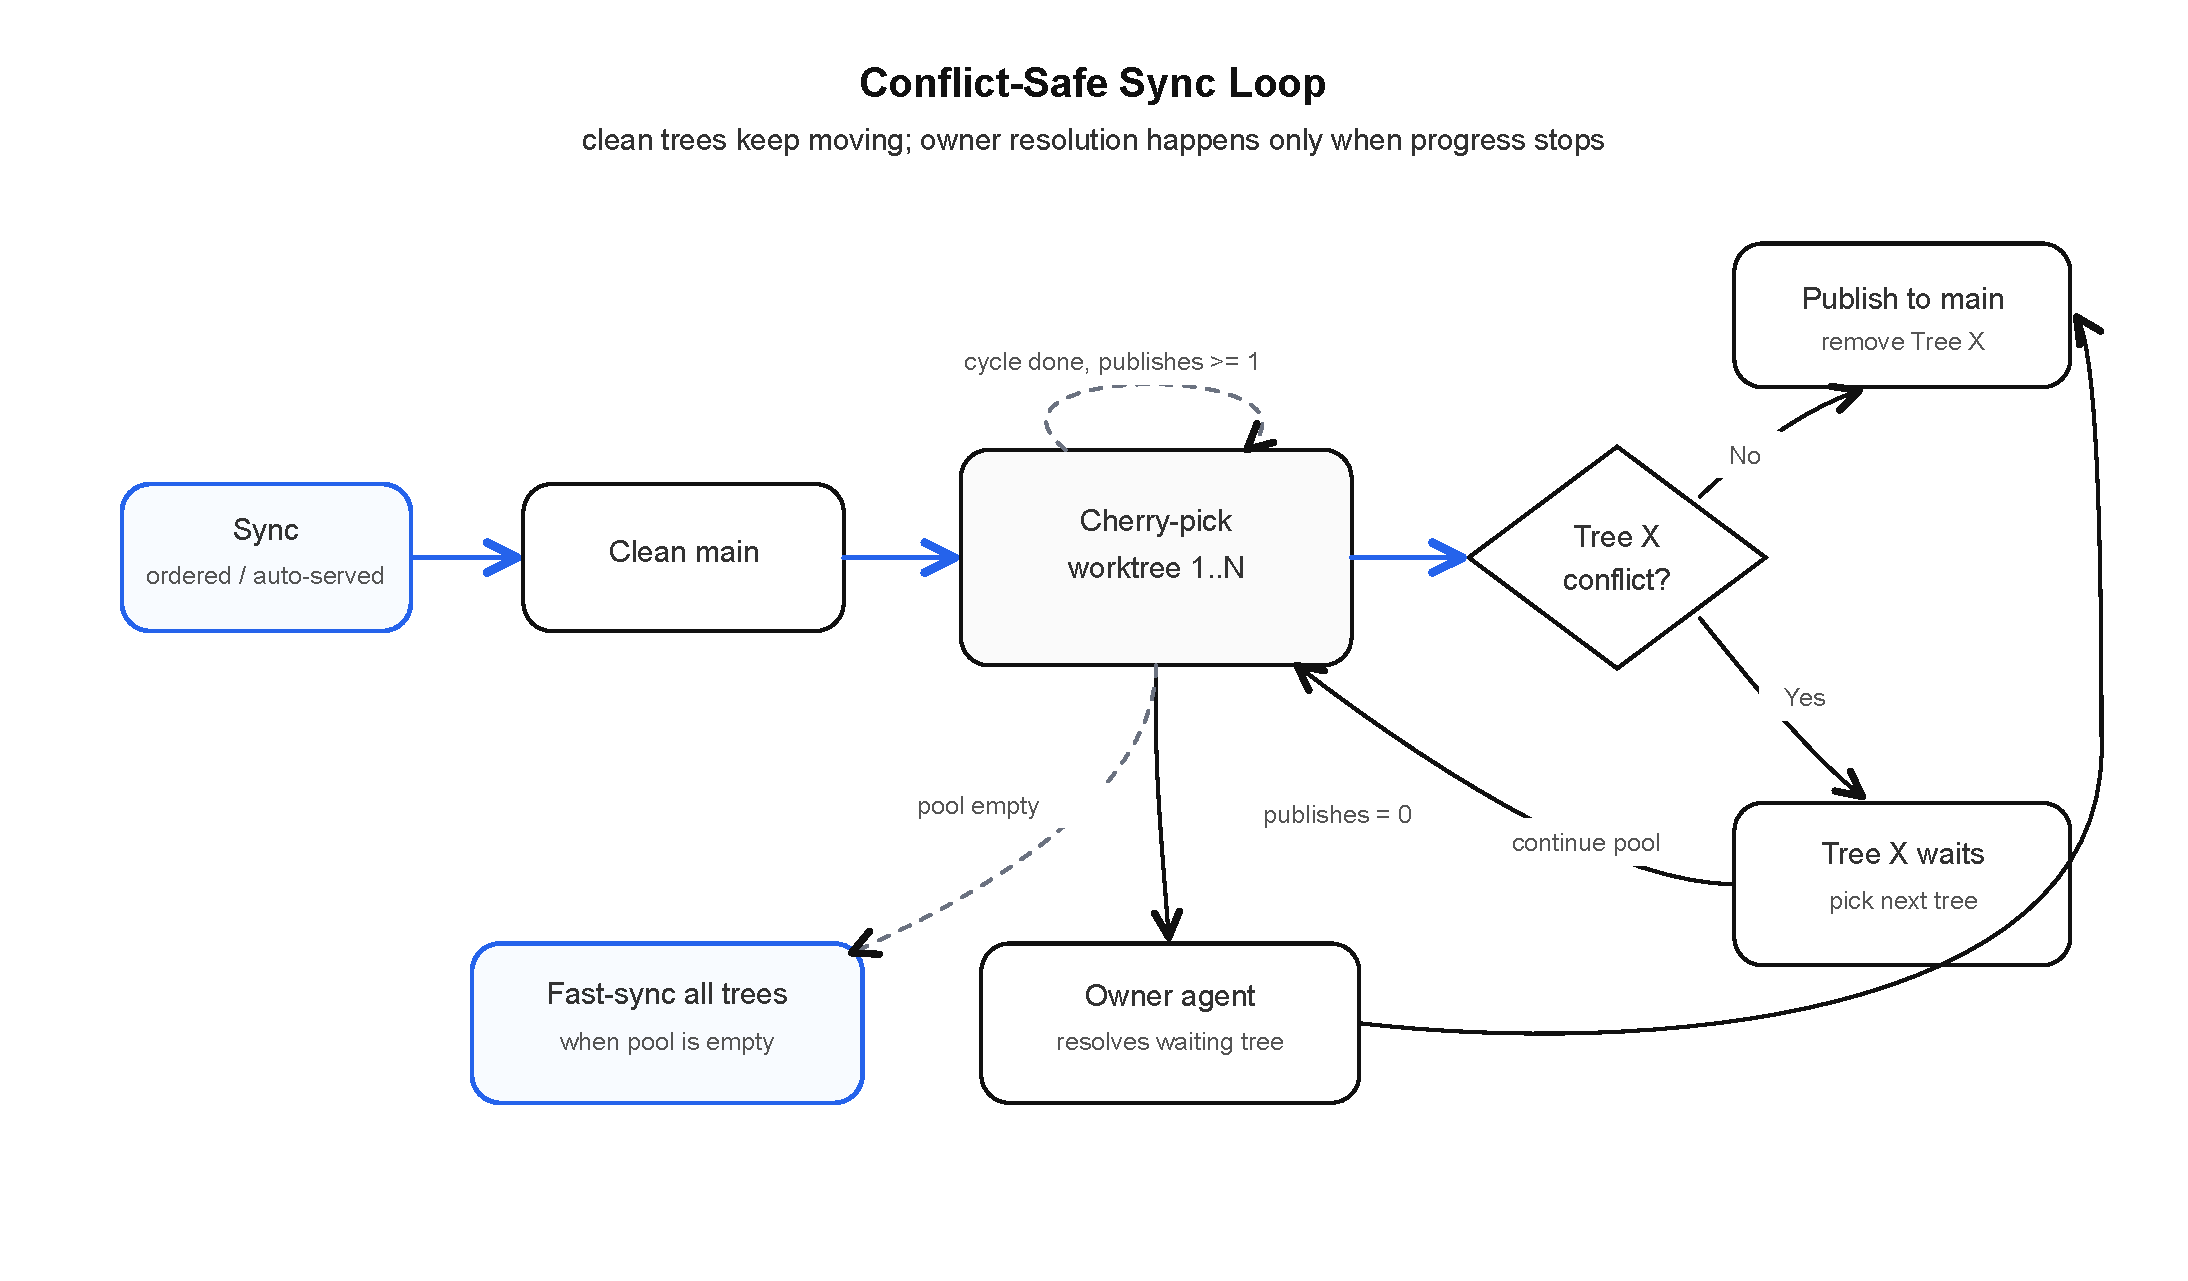
\includegraphics[width=\textwidth,height=0.78\textheight,keepaspectratio]{Fig1.pdf}
\caption{One synchronization round as a loop. Reproduced from the Kota whitepaper \citep{wu2026kotalongtermteammates}.}\label{fig:sync-loop}
\end{figure}
\section{Performance analysis}\label{sec:performance}

This section gives the arithmetic behind the two claims: what a synchronization costs when nothing conflicts, what clean-first scheduling changes when something does, and how delay---before a conflict is detected and before it is repaired---inflates the work. Each result states the assumptions it needs. Where the assumptions stop, Section~\ref{sec:verification} measures.

\subsection{With no conflicts, synchronization adds no repair and no retry}\label{sec:no-conflicts}

\textbf{Claim.} If at least one commit is pending and no pending commit conflicts with the base or with any other pending commit, a Bartender round integrates exactly the commits that one-by-one integration in the same order would integrate, in the same order, producing the same shared-branch content; it finishes in one pass with no repair and no retry. Counted as worktree attempts or as commit applications, the integration work is identical.

\textbf{Proof sketch.} With no conflicts, every cherry-pick of the first pass succeeds, so nothing remains for a second pass; the sequence of applications is the baseline's, and induction over it gives the same file tree and the same count (Appendix~\ref{app:equivalence}, clean integration).

What the round adds beyond that work is Git bookkeeping---scanning, snapshotting, refreshing worktrees, locking. None of it involves an agent: no tokens, no author time. Synchronizing often therefore costs machine time, and nothing else, as long as nothing conflicts. Two remarks: equal content does not mean equal commit identifiers, which depend on parents and metadata; and the bookkeeping is repeated every round, so it is cheap, not zero.

\subsection{With conflicts: clean work never waits, and no more items need repair}\label{sec:repair-order}

Compare Bartender's schedule---integrate everything clean, hold what conflicts, repair the held items afterwards---with \emph{in-place repair}: process worktrees in order and, on a conflict, repair it before moving on. In-place repair is an analysis baseline that stands in for its real-world counterpart, merging single worktrees on demand, which is common in both AI-assisted and human-only development.

\textbf{Clean work never waits.} Call \emph{C} the items that land during Bartender's automatic pass. Every item in \emph{C} lands without waiting for any author repair. Under in-place repair, the same item waits for the repair durations of the conflicting items before it; if an earlier repair poisons it, it becomes dirty, and its own repair time is added as well. A repair takes minutes; an integration attempt takes seconds. Both schedules pay their own total attempt time plus their own total repair time (Appendix~\ref{app:clean-items}, waiting).

\textbf{No more items need repair.} Table~\ref{tab:repair-example} works through four worktrees A--D, processed in that order, each standing for one indivisible pending patch; A and C apply cleanly to the base and to each other, B and D conflict with the base.

\begin{table}[tbp]
\caption{Four worktrees under the two schedules.}\label{tab:repair-example}
\centering\small
\setlength{\tabcolsep}{4pt}
\renewcommand{\arraystretch}{1.12}
\begin{tabularx}{\textwidth}{@{}lXcX@{}}
\toprule
Policy & Sequence of events & Repairs & Items already landed at each repair \\
\midrule
In-place repair & A lands; B repaired; C, poisoned by the repaired B, repaired; D repaired & 3 & \{A\}; \{A, B\}; \{A, B, C\} \\
\addlinespace[3pt]
Bartender & A and C land; B repaired; D repaired & 2 & \{A, C\}; \{A, C, B\} \\
\bottomrule
\end{tabularx}
\end{table}

\begin{figure}[tbp]
\centering
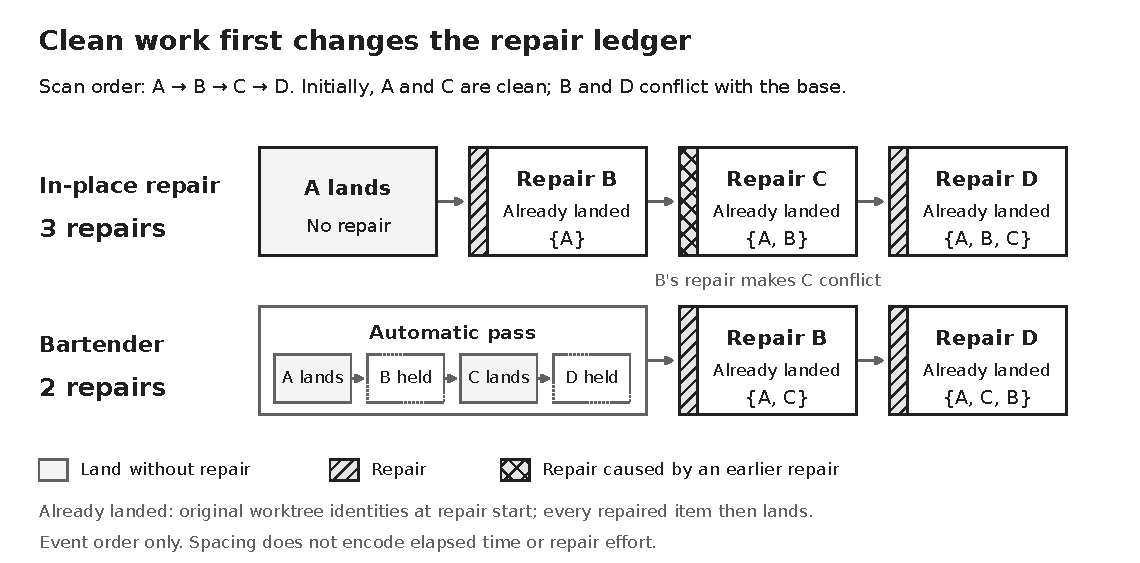
\includegraphics[width=\textwidth,height=0.78\textheight,keepaspectratio]{Fig2.pdf}
\caption{The four-worktree example as two event lines. Each repair lists the worktrees already landed when it starts; under in-place repair the repaired B poisons C. Event order only.}\label{fig:repair-order}
\end{figure}

The example generalizes under a declared model: a fixed batch of indivisible items in a fixed order, so a worktree with several commits is outside the model; whether two original items conflict is decided by the intersection of immutable footprints, with no rescue by dependency or by identical content; more content in the base never removes a conflict; a repaired item keeps its footprint exactly; each item that needs repair is repaired exactly once and lands immediately.

\emph{Repaired sets.} An item that is clean in Bartender's pass faces only the clean items before it; under in-place repair the same item faces every earlier item and every earlier repair. Its context is a superset, so if it conflicts under Bartender it conflicts under in-place repair. Writing R for the set of items that need an author repair, \[
R_{\text{Bartender}} \subseteq R_{\text{in-place}}, \qquad |R_{\text{Bartender}}| \le |R_{\text{in-place}}|,
\]

with strict inequality whenever an in-place repair poisons a later clean item, as the repaired B poisons C in Table~\ref{tab:repair-example} (Appendix~\ref{app:repair-sets}, repair sets).

\emph{Context of a shared repair.} For an item repaired under both schedules, the set of original items already landed when its repair begins is, under Bartender, the in-place set plus the clean items that follow it in the original order; the two coincide only when no clean item follows. This concerns which items have landed, not the realized footprint of their repairs, the Git content, or the difficulty of the repair.

\emph{Net effort.} Bartender repairs no more items, and sometimes fewer; each shared repair faces no smaller landed set. Whether total effort is lower depends on how much poisoning occurs, which depends on overlap density; even within the model, examples go both ways (Appendix~\ref{app:total-effort}, total effort). Section~\ref{sec:verification} measures it, under the stated assumption that a larger landed set means a harder repair.

\textbf{Boundary.} If repairs may shrink their footprint, the subset claim fails. Take base \{x\}; A = \{x, y\}, B = \{y, z, w\}, C = \{z\}, D = \{w\}. Bartender lands only B in the first pass, with its full footprint, and repairs A, C, and D; in-place repair repairs A, then B, which shrinks to \{y\}, after which C and D land cleanly---three repairs against two. When a repair may shrink its effective footprint, the clean item that landed first poisons later ones with its full footprint. The claim therefore requires footprint-preserving repairs (Appendix~\ref{app:counterexamples}, counterexamples).

\textbf{Shipped behavior.} Within one round, the implementation holds conflicting worktrees, integrates the rest, retries failed worktrees while progress continues, and on stalling dispatches the first conflict and returns. ``All conflicts repaired in sequence'' is realized across rounds, as authors repair and re-trigger synchronization; the analysis treats it as that protocol.

\subsection{The cost of delay}\label{sec:delay}

\textbf{Conflicts arise only between concurrent edits, and synchronization turns concurrency into sequence.} Delay enters twice: time passes before a conflict is detected, and time passes before anyone---agent or human---starts to repair it. We call the first the synchronization interval (\(\tau\)) and the second the wait after dispatch (\(\delta\)).

An example. Two agents, A and B, work on the same project. A edits lines 10--20 of \texttt{auth.rs} on Monday; B's task touches lines 15--25. Synchronized daily, B starts on Tuesday from a base that already contains A's change, and the overlap is at most one small hunk, repaired the same day. Synchronized weekly, the same overlap surfaces on Friday entangled with a week of other changes. On the second axis: a conflict detected at ten is repaired at once against a fresh base; noticed two days later, it is repaired against two days of other agents' work and may be ejected again on re-submission.

\begin{figure}[tbp]
\centering
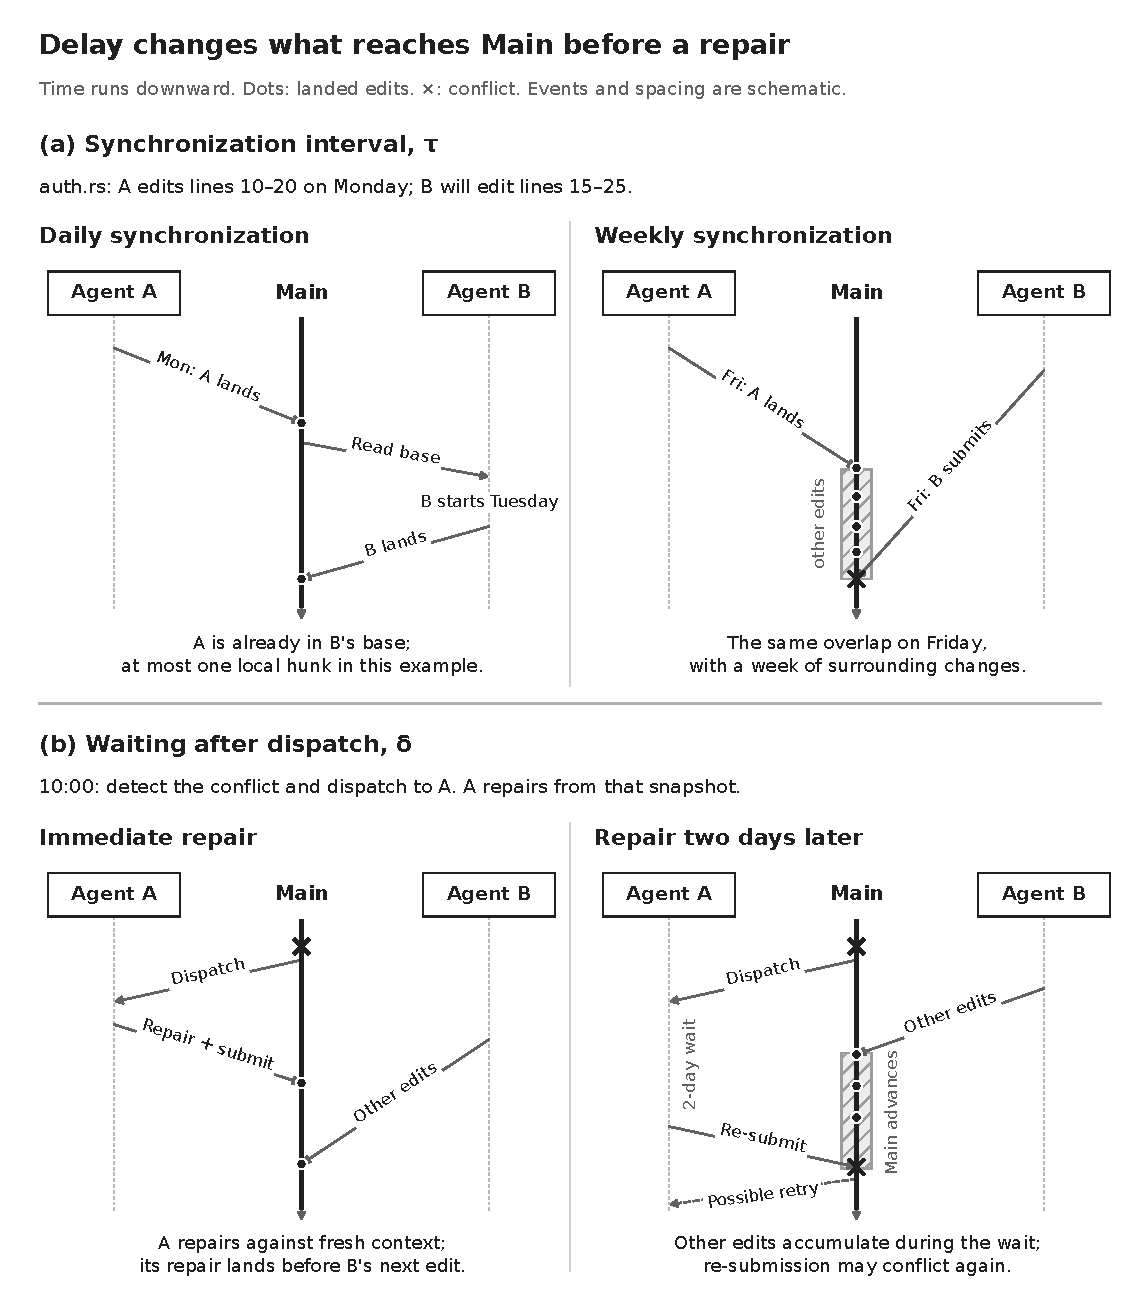
\includegraphics[width=\textwidth,height=0.78\textheight,keepaspectratio]{Fig3.pdf}
\caption{Delay along the shared branch. Main sits between Agent A and Agent B, time runs downward; arrows are integrations, base reads, or handbacks, dots landed edits, crosses conflicts, hatched segments accumulated context. (a) Daily against weekly synchronization. (b) Repair at once against repair two days after dispatch. Schematic, not measured.}\label{fig:delay-context}
\end{figure}

\textbf{Synchronization interval.} Each agent accumulates about \(\lambda \tau\) edits per interval, so the expected number of overlapping pairs between two agents per synchronization is \(p(\lambda \tau )^2\). Across all agents, \[
\begin{aligned}
\text{overlapping pairs per synchronization} &\approx \binom{n}{2}\, p\, \lambda^2 \tau^2, \\
\text{overlapping pairs per unit time} &\approx \binom{n}{2}\, p\, \lambda^2 \tau .
\end{aligned}
\]

This counts overlapping concurrent pairs of edits, not detected conflicts or repair events; one edit may overlap several others. The rate grows with \(\tau\) even per unit time---linearly here, strictly whenever \(n\) ≥ 2, \(p\) \textgreater{} 0, and \(\lambda\) \textgreater{} 0 (Appendix~\ref{app:overlap-pairs}, pair counts). If repair cost grows with the neighboring edits a conflict is entangled with---a modeling assumption---then that context also grows about linearly in \(\tau\), and the conflict mass per synchronization grows faster than the count. This is the first-order account of the ``enormous rebase'' of infrequent merging.

\textbf{Waiting after dispatch.} During a repair's exposure \(E\), other agents land edits overlapping the conflicting region at rate \(\mu\), so the context the repair must reconcile grows linearly in \(E\), and the probability that the re-submitted commit collides with something landed meanwhile is \[
q = 1 - e^{-\mu E} .
\]

A collision sends the commit back for another attempt; with independent attempts, the expected number of attempts is

\[
\frac{1}{1-q} = e^{\mu E} .
\]

Expected attempts grow exponentially with exposure; there is no finite threshold, and the characteristic scale is 1/\(\mu\), at which the expected number of attempts is about \(e\) (Appendix~\ref{app:exposure}, repeated attempts). Immediate dispatch removes the queue wait \(Q\). At the intended operating point the author also starts at once, \(\delta\) ≈ 0, and with the base as of dispatch the exposure is about \(R\); this is a condition of the model, not a measured response-time guarantee, and how short \(R\) is in practice is not measured here. Re-reading the base when repair begins shortens the collision window to about \(R\) while the context still grows over \(\delta\). Within a finite observation window the paper reports the \emph{finite-window unresolved fraction}, the share of conflicts not landed by the window's end; it is not evidence of permanent starvation (Appendix~\ref{app:finite-window}, finite window).

\textbf{Symbols.} The quantities used above are:

\begin{center}
\centering\small
\setlength{\tabcolsep}{4pt}
\renewcommand{\arraystretch}{1.12}
\begin{tabularx}{\textwidth}{@{}l>{\raggedright\arraybackslash}X@{}}
\toprule
Symbol & Meaning \\
\midrule
\(n\) & number of agents \\
\addlinespace[3pt]
\(\lambda\) & edits per agent per unit time, as a Poisson process \\
\addlinespace[3pt]
\(p\) & probability that two edits by different agents overlap \\
\addlinespace[3pt]
\(\tau\) & synchronization interval \\
\addlinespace[3pt]
\(Q\) & queue wait from a conflict's detection to its dispatch (the shipped implementation dispatches one conflict per round) \\
\addlinespace[3pt]
\(\delta\) & author's delay from dispatch to the start of repair \\
\addlinespace[3pt]
\(R\) & duration of a repair \\
\addlinespace[3pt]
\(E\) & exposure of a repair: \(E = \delta  + R\) with the base as of dispatch; \(E = Q + \delta  + R\) with the base as of detection; \(E = R\) with the base re-read when repair starts \\
\addlinespace[3pt]
\(\mu\) & rate at which other agents land edits overlapping a given region; when their edits land promptly at rate (\(n\)−1)\(\lambda\) and each overlaps the region independently with probability \(p\), \(\mu  = p(n-1)\lambda\) \\
\addlinespace[3pt]
\(q\) & probability that a re-submitted repair collides with an edit landed during its exposure \\
\bottomrule
\end{tabularx}
\end{center}

The two axes differ: \(\tau\) determines how many conflicts arise and how large they are; \(E\) determines how many attempts one conflict takes and how much context each faces. The first supports claim one, the second claim two.

In sum: a conflict-free round does exactly the baseline's integration work; under clean-first scheduling, clean items never wait, and in a fixed batch with footprint-preserving repairs no more items need repair than under in-place repair; under independence assumptions, overlapping pairs grow linearly with the synchronization interval per unit time, and expected repair attempts grow exponentially with exposure. Total repair effort, and whether these shapes survive relaxed assumptions, are left to Section~\ref{sec:verification}.
\section{Verification and simulation}\label{sec:verification}

This section answers two questions. Does the shipped code behave as Section~\ref{sec:mechanism} describes? And do the conclusions of Section~\ref{sec:performance}, which rest on strong assumptions, survive when those assumptions are relaxed toward realistic conditions---and how large are the effects? Both were executed on 9 September 2026: the conformance scenarios against the released application, and the simulation as 29,700 runs.

\subsection{Conformance of the implementation}\label{sec:conformance}

\textbf{What it establishes.} That the steps of Section~\ref{sec:mechanism} are the actual behavior of the released application, not a reading of its documentation. The scenarios observe the application from outside---Git state of the shared branch and worktrees, the request receipt, and the actor's event log---with the authoring roles bound to a disabled provider, so they test routing and recording, not repair by a live agent.

\textbf{Execution.} The application under test was release v0.1.10 (public commit \texttt{75eb8fda}), whose backend source tree is identical to the audited commit of Section~\ref{sec:mechanism}; the installed application and its bundled command-line tool were hashed against the published release assets. Four scenarios were run, each on two fresh fixtures, each fixture receiving one synchronization request and then a second request with no intervening edit: eight fixture executions and sixteen requests. Before every request the fixture's initial Git state, role mapping, and provider files were re-checked.

\begin{table}[tbp]
\caption{Conformance observations. ``Published'' is the number of commits integrated by the request; ``conflicts'' is the number reported.}\label{tab:conformance}
\centering\small
\setlength{\tabcolsep}{4pt}
\renewcommand{\arraystretch}{1.12}
\begin{tabularx}{\textwidth}{@{}>{\raggedright\arraybackslash}p{0.24\textwidth}*{4}{>{\raggedright\arraybackslash}X}@{}}
\toprule
Scenario & Published, request 1 / 2 & Conflicts, request 1 / 2 & Repetitions & Outcome \\
\midrule
One clean worktree & 1 / 0 & 0 / 0 & 2 & as specified \\
\addlinespace[3pt]
Three clean worktrees & 3 / 0 & 0 / 0 & 2 & as specified \\
\addlinespace[3pt]
One clean, one conflicting & 1 / 0 & 1 / 1 & 2 & as specified \\
\addlinespace[3pt]
One clean, two conflicting & 1 / 0 & 2 / 2 & 2 & as specified \\
\bottomrule
\end{tabularx}
\end{table}

All sixteen requests completed with every fixed assertion satisfied. Clean worktrees were integrated on the first request and nothing on the second. Conflicting worktrees were held; the clean worktree in the same request was integrated; a repair notice was recorded for the first blocked role only, with delivery marked skipped because the role's provider was disabled; the second request left the Git state and the notice identifiers unchanged. These observations cover steps 1, 2, 4, and 5 of Section~\ref{sec:mechanism} at the level visible from outside the application. They do not show delivery to a live agent, a successful repair, internal pass counts, or worktree-level atomicity, and six further scenarios---multi-commit prefixes, identical changes, dependency-driven retry, a pass with no progress, dirty worktrees, and inactive or unreachable authors---were not executed.

\subsection{Behavior under more realistic conditions}\label{sec:simulation}

The first-order model of Section~\ref{sec:performance} assumes independent edits, uniform overlap, footprint-preserving repairs, and no rescue. The simulation relaxes these and asks whether the two claims survive: does frequent synchronization still pay, and does immediate repair by the owning agent still pay, when edits depend on each other, files are finite, and repairs take time?

\textbf{Environment.} The simulation is a discrete-event script with no real code and no language model: both questions concern when edits overlap and when they are concurrent, not code semantics. Code is abstracted to line intervals on files; two edits overlap when their intervals intersect on the same file. The world has \(K\) files of \(L\) lines and \(n\) agents, each producing edits as a Poisson process with rate \(\lambda\); an edit is a random interval on a random file. Two factors make it more realistic than the first-order model: \emph{dependency}---with probability \(d\) an edit depends on another agent's recent edit and cannot apply until that edit has landed, the case that mechanical retry rescues---and \emph{finite files}, which bound conflict growth. A repair takes time \(R\) and preserves its footprint; rescue by identical content is not modeled. Three policies replay the same edit stream from the same seed, so differences come from policy alone: \emph{Bartender} (integrate clean worktrees, hold conflicts, dispatch to the author at once); \emph{in-place repair} (process in order, repair each conflict before moving on; the baseline of Section~\ref{sec:performance}); and \emph{kick-back} (eject the conflicting worktree, whose author returns after \(\delta\); Bartender without immediate dispatch). The simulation lives in a separate research repository and does not modify Kota; seeds and configurations are fixed, so runs are reproducible. Table~\ref{tab:parameters} lists the parameters; all values were fixed before any run.

\begin{table}[tbp]
\caption{Simulation parameters. Time is measured in units of one agent's mean inter-edit time.}\label{tab:parameters}
\centering\small
\setlength{\tabcolsep}{4pt}
\renewcommand{\arraystretch}{1.12}
\begin{tabularx}{\textwidth}{@{}>{\raggedright\arraybackslash}p{0.14\textwidth}*{3}{>{\raggedright\arraybackslash}X}@{}}
\toprule
Symbol & Meaning & Stands for & Values \\
\midrule
\(n\) & agents & team size & 2, 4, 8 \\
\addlinespace[3pt]
\(\lambda\) & edits per agent per unit time & development pace & 1 (the unit) \\
\addlinespace[3pt]
\(K\), \(L\) & files, lines per file & codebase size & 8, 256 \\
\addlinespace[3pt]
edit length & lines per edit; determines \(p\) & how crowded the codebase is & 4, 16, 64 lines → \(p\) ≈ 0.0034, 0.0156, 0.0687 \\
\addlinespace[3pt]
\(d\) & probability that an edit depends on another agent's recent edit & task coupling & 0, 0.1, 0.3 \\
\addlinespace[3pt]
\(\tau\) & synchronization interval & idle-, agent-, and user-triggered regimes & 0.125, 0.25, 0.5, 1, 2, 8, 32 \\
\addlinespace[3pt]
\(\delta\) & author's delay after dispatch & Bartender ≈ 0; human review, hours to days & 0, 0.25, 0.5, 1, 2, 4 × 1/μ \\
\addlinespace[3pt]
\(R\) & repair duration & agent repair time & 0.25, or 0.25 + 0.05 per unseen foreign landed edit \\
\addlinespace[3pt]
seeds & replications per cell & --- & 30 \\
\addlinespace[3pt]
window & observation window & --- & max(256, 32/μ) \\
\bottomrule
\end{tabularx}
\end{table}

\textbf{Execution.} 990 cells, each replicated over 30 seeds: 29,700 runs, executed serially on one machine in 100 minutes with no failed run. An order-sensitive comparison in the verification tool first held the delivery; after the tool was corrected to compare rows as multisets, the preserved outputs were re-verified without regeneration. Intervals are means ± 1.96 × sample standard deviation / \(\sqrt{30}\) across seeds; ratios of pooled totals carry no interval.

\textbf{Result 1: fewer repairs and far less repair work.} The same edit stream, synchronized every unit of time, under Bartender and under in-place repair, across the three overlap levels and five team slices. \emph{Result.} Table~\ref{tab:repair-comparison} and Figure~\ref{fig:repairs-overlap}. At low overlap the two schedules are indistinguishable. At high overlap in-place repair needs 2.8 times as many repairs and 12 times as much repair work as Bartender with four agents, and 2.5 times as many repairs and 29 times as much work with eight. When edits depend on each other, in-place repair saturates near the window's capacity while Bartender stays well below it. Across all 315 paired cells, Bartender's mean repair count is lower in 259, equal in 49, and higher in 7; the seven reversals are dynamic cells, outside the fixed-batch conditions of Section~\ref{sec:repair-order}. \emph{Conclusion.} The clean-first schedule of Section~\ref{sec:repair-order} is not only provably no worse in a fixed batch; under dynamic conditions its advantage grows with overlap and with coupling, and the effort gap is an order of magnitude at the high end.

\begin{table}[tbp]
\caption{Repairs and repair work per run at synchronization interval 1 (means over 30 seeds; effort counts the landed edits each repair had to reconcile).}\label{tab:repair-comparison}
\centering\small
\setlength{\tabcolsep}{4pt}
\renewcommand{\arraystretch}{1.12}
\begin{tabularx}{\textwidth}{@{}l r *{2}{>{\raggedright\arraybackslash}X}@{}}
\toprule
Agents, dependency & Overlap \(p\) & Repairs: Bartender / in-place & Repair work: Bartender / in-place \\
\midrule
4, 0 & 0.0034 & 4.9 / 5.0 & 8.5 / 8.5 \\
\addlinespace[3pt]
4, 0 & 0.0156 & 24.4 / 26.9 & 41 / 45 \\
\addlinespace[3pt]
4, 0 & 0.0687 & 100.7 / 281.1 & 176 / 2,137 \\
\addlinespace[3pt]
8, 0 & 0.0034 & 22.3 / 25.6 & 44 / 50 \\
\addlinespace[3pt]
8, 0 & 0.0156 & 100.4 / 456.7 & 192 / 7,154 \\
\addlinespace[3pt]
8, 0 & 0.0687 & 395.3 / 1,004.4 & 840 / 24,167 \\
\addlinespace[3pt]
4, 0.3 & 0.0687 & 628.5 / 973.0 & 660 / 982 \\
\bottomrule
\end{tabularx}
\end{table}

\begin{figure}[tbp]
\centering
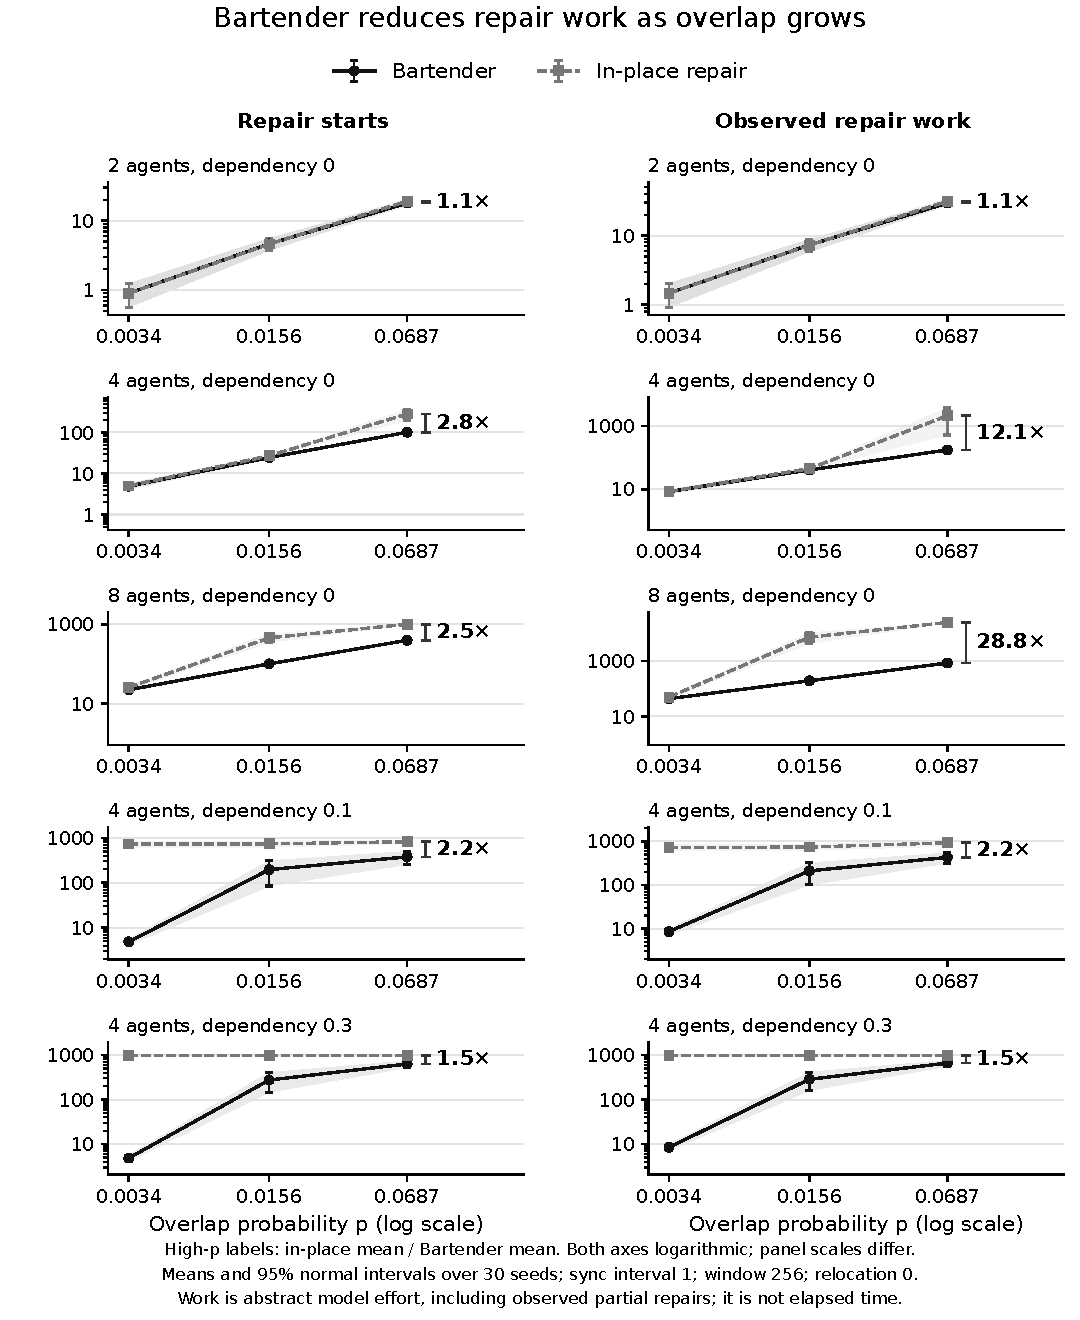
\includegraphics[width=\textwidth,height=0.78\textheight,keepaspectratio]{Fig4.pdf}
\caption{Repairs and repair work against overlap probability, Bartender against in-place repair, for five team slices; synchronization interval 1. Both axes are logarithmic; labels give the in-place to Bartender ratio at the highest overlap.}\label{fig:repairs-overlap}
\end{figure}

\textbf{Result 2: longer synchronization intervals mean more and larger conflicts.} Sweep the interval \(\tau\) from 0.125 to 32 with four agents and no dependency; count overlapping concurrent pairs per unit time, first conflicts per unit time, and the overlap at the first conflict. \emph{Result.} Figure~\ref{fig:sync-interval}. The rate of overlapping pairs follows the first-order line \(C(n,2)\cdot p\cdot\lambda^2\cdot\tau\) over the whole sweep, and lies above it at the largest interval for 64-line edits (16.1 against 13.2 pairs per unit time at \(\tau\) = 32). First conflicts per unit time rise from 0.055 to 2.14 for 64-line edits, and the overlap at the first conflict grows from 34 to 57 lines; for 4-line edits the overlap cannot grow and stays near 2.4 lines. \emph{Conclusion.} Delay before detection costs linearly in conflict count and, for edits large enough to entangle, also in conflict size. Bartender's idle-triggered rounds sit at the small-\(\tau\) end of this axis; on-demand merging sits at the large end.

\begin{figure}[tbp]
\centering
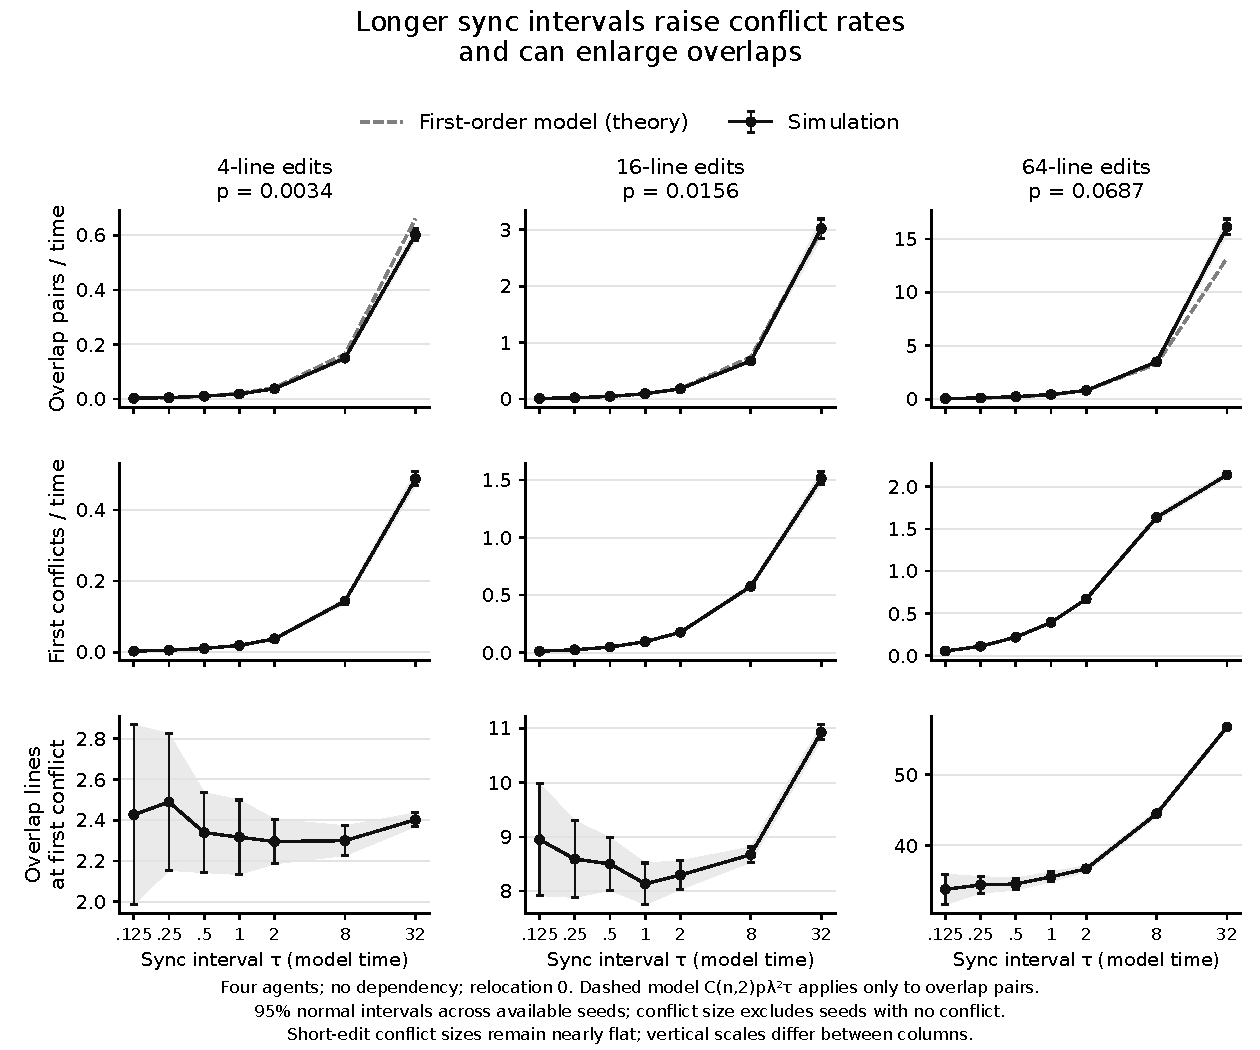
\includegraphics[width=\textwidth,height=0.78\textheight,keepaspectratio]{Fig5.pdf}
\caption{Overlapping concurrent pairs per unit time (with the first-order line), first conflicts per unit time, and overlap at the first conflict, against the synchronization interval; four agents, no dependency; columns are the three edit lengths.}\label{fig:sync-interval}
\end{figure}

\textbf{Result 3: waiting before repair fails more re-submissions and leaves conflicts unresolved.} Under kick-back, sweep the author's wait \(\delta\) from 0 to four times 1/\(\mu\), where 1/\(\mu\) is the characteristic time between landings of edits that overlap a given region (for four agents and 16-line edits, 1/\(\mu\) ≈ 21 units, so 4/\(\mu\) ≈ 85 units). A repair is modeled, not performed: after the wait, the author produces a patch with the same footprint against a base and re-submits it; the re-submission fails if another agent landed an overlapping edit between that base and the re-submission. Two variants of the base are run: the base as of dispatch, and the base re-read when the repair starts. Four agents, no dependency, fixed \(R\). \emph{Result.} Table~\ref{tab:wait-outcomes} and Figures~\ref{fig:wait-resolved}--7. At the modeled zero-wait point---immediate dispatch with the author starting at once, Bartender's intended operating point---virtually every initial conflict lands within the window (99.8--100 percent across the three edit lengths). As the wait grows, the share that lands falls, to 27--52 percent at 4/\(\mu\) with the dispatch-time base and 70--79 percent with re-reading. The cause is in Figure~\ref{fig:wait-failures}: the fraction of completed repair attempts that fail on re-submission rises from zero to 73--84 percent with the dispatch-time base---following the first-order \(q\) in shape and below it in magnitude (98 percent)---while re-reading keeps it under two percent, because its exposure is only \(R\). What re-reading cannot recover is the window's capacity: a single repair slot with long waits completes only seven to thirteen repairs per window, so conflicts queue and part of them never land. \emph{Conclusion.} Delay before repair costs twice---through collisions when the repair uses a stale base, and through queueing whatever base it uses---and only repairing at once, with no wait after dispatch, avoids both. The mean number of re-dispatch rounds, which the first-order model puts at exp(\(\mu E\)), is not reported: in a finite window with a single repair slot that mean is truncated by the queue and is not identifiable, so the exponential law is neither confirmed nor refuted here.

\begin{table}[tbp]
\caption{Outcome of a conflict against the author's wait, for 16-line edits (four agents, no dependency, fixed R). Landed: share of initial conflicts resolved within the window. Failed: share of completed repair attempts that collided on re-submission. Ranges across the three edit lengths are given in the text.}\label{tab:wait-outcomes}
\centering\small
\setlength{\tabcolsep}{4pt}
\renewcommand{\arraystretch}{1.12}
\begin{tabularx}{\textwidth}{@{}l *{2}{>{\raggedright\arraybackslash}X}@{}}
\toprule
Wait \(\delta\) (× 1/μ) & Base as of dispatch: landed / failed & Base re-read at repair: landed / failed \\
\midrule
0 (Bartender model) & 100\% / 0\% & 100\% / 0\% \\
\addlinespace[3pt]
0.25 & 97\% / 9\% & 98\% / 1\% \\
\addlinespace[3pt]
0.5 & 94\% / 19\% & 95\% / 1\% \\
\addlinespace[3pt]
1 & 87\% / 33\% & 91\% / 0\% \\
\addlinespace[3pt]
2 & 68\% / 57\% & 83\% / 0\% \\
\addlinespace[3pt]
4 & 33\% / 78\% & 70\% / 1\% \\
\bottomrule
\end{tabularx}
\end{table}

\begin{figure}[tbp]
\centering
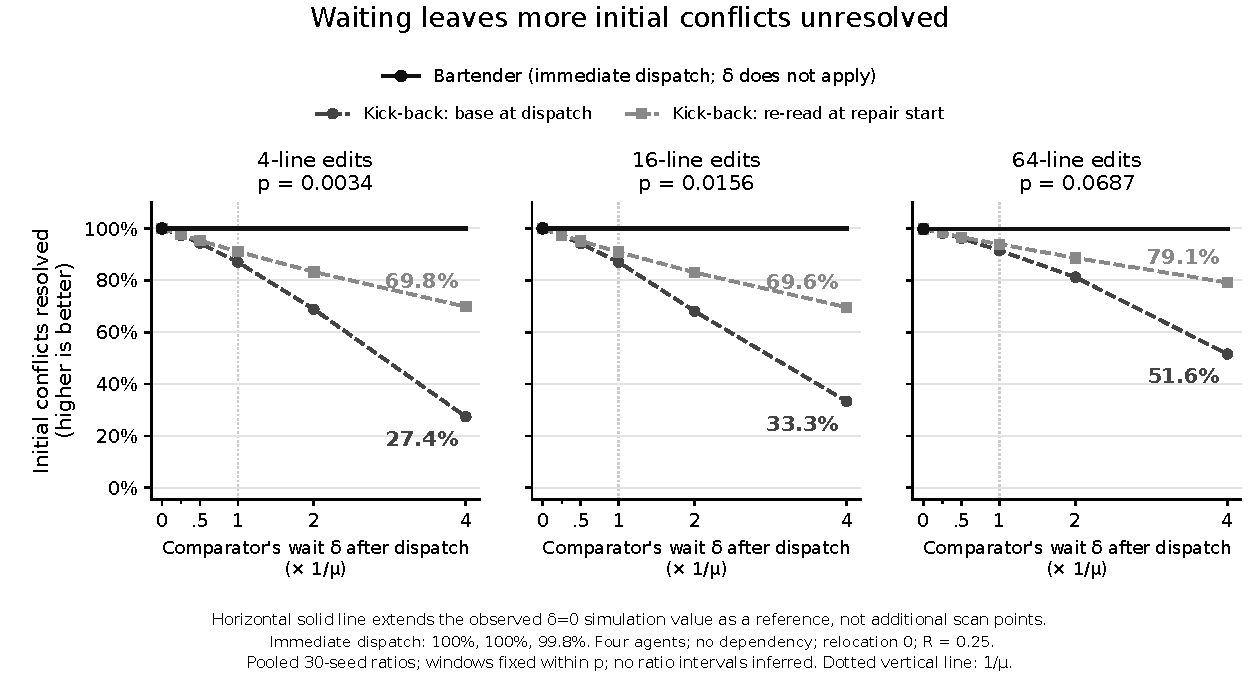
\includegraphics[width=\textwidth,height=0.78\textheight,keepaspectratio]{Fig6.pdf}
\caption{Share of initial conflicts resolved within the window against the comparator's wait after dispatch; four agents, no dependency, fixed repair clock; columns are the three edit lengths. Dashed: kick-back with the base as of dispatch or re-read at repair start. Solid: the modeled zero-wait point (immediate dispatch, author starting at once), Bartender's intended operating point; the line extends its observed zero-wait value for comparison.}\label{fig:wait-resolved}
\end{figure}

\begin{figure}[tbp]
\centering
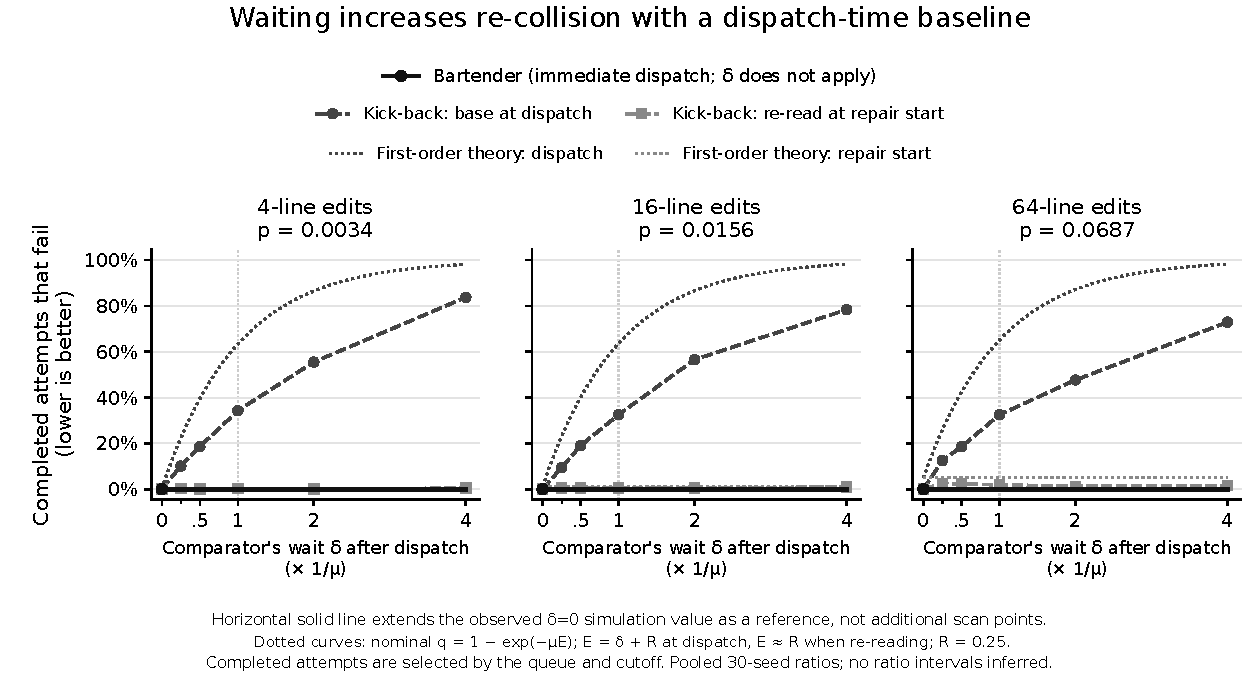
\includegraphics[width=\textwidth,height=0.78\textheight,keepaspectratio]{Fig7.pdf}
\caption{Share of completed repair attempts that fail on re-submission against the comparator's wait, with the first-order q for each variant as dotted lines. Solid: Bartender's observed zero-wait value, extended for comparison.}\label{fig:wait-failures}
\end{figure}

\textbf{What the simulation shows.} Three results, with their conditions. First, against in-place repair on the same edit stream, Bartender's clean-first schedule needs fewer repairs and far less repair work, and the gap grows with overlap and with coupling: at the highest overlap, in-place repair needs 2.8 times as many repairs and 12 times as much work with four agents, and 2.5 times as many repairs and 29 times as much work with eight; when a tenth of edits depend on another agent's recent edit, in-place repair spends its window on about 730 repairs regardless of overlap, while Bartender's retry after progress resolves most dependency failures without an author and needs 5 repairs at low overlap and 380 at high. At low overlap without coupling the two schedules are equal. Second, synchronizing more often lowers both the rate and the size of conflicts: over the sweep from an interval of 32 down to 0.125, the rate of first conflicts fell by a factor of 39 and their size fell by 40 percent for 64-line edits, in line with the first-order law. Third, dispatching a conflict to its author at once keeps virtually every conflict resolvable within the window, whereas waiting four characteristic times before repair left 48--73 percent unresolved with a stale base and 21--30 percent even with a fresh one, because 73--84 percent of re-submissions collided and the repair queue filled. These are model quantities under the parameters of Table~\ref{tab:parameters}, not measurements of the product.

\textbf{Rules that were followed.} Sweep ranges were fixed before running; every cell has thirty seeds; normalization is by equal observation period and equal total edits; no parameter was selected after the fact. Two expectations fixed before the runs did not appear and are reported as such: the pair rate did not flatten within the sweep, and a knob that let an agent relocate an edit overlapping a visible landed edit brought no consistent reduction in conflicts at any setting; it is dropped from the account above and kept in the supplementary figures. We did not replay real Git history with synchronization artificially delayed to session end. Deliverables: simulation code, configurations, seeds, per-cell aggregates for all 990 cells, the paired differences, the hash of the raw-record archive, and supplementary figures covering every slice of the sweep, including flat and unfavorable results, released with the paper.
\section{Deployment record}\label{sec:deployment}

The mechanism's own deployment is Kota's development workspace. The record covers 1 June to 9 September 2026, UTC, end exclusive (100 days), from the first complete month after the synchronization backend entered the Git history to the last complete day before extraction. The sources are retained command-line request/result pairs, the Bartender actor's handoff log, and reachable main-branch Git history \citep[Bartender deployment records,][]{bartender-deployment-records}; software and logging changed during the window, so the record spans several versions rather than the pinned commit of Section~\ref{sec:mechanism}. Rounds started from the application leave no receipt, so receipt-based counts cover command-line rounds only: no overall count of rounds exists, and neither a success rate nor a conflict rate can be estimated. Table~\ref{tab:deployment} lists what the records show.

\begin{table}[tbp]
\caption{What the retained records show.}\label{tab:deployment}
\centering\small
\setlength{\tabcolsep}{4pt}
\renewcommand{\arraystretch}{1.12}
\begin{tabularx}{\textwidth}{@{}>{\raggedright\arraybackslash}p{0.24\textwidth}*{2}{>{\raggedright\arraybackslash}X}@{}}
\toprule
Record set & Observed & Meaning \\
\midrule
Participants & at least 10 worktree/agent identities, pseudonymized W01--W10 & union of receipt, snapshot, and handoff evidence; no current-roster filter, so departed identities are kept; not a count of people \\
\addlinespace[3pt]
Paired command-line rounds & 82, all reporting success & 67 published commits and 15 published none; 176 commit operations and 5 snapshot operations; initiator unknown for all 82 \\
\addlinespace[3pt]
Agent snapshot commits on main & 158 & mechanical snapshots; not rounds, and not additive with the 82 \\
\addlinespace[3pt]
Conflict handoffs & 3 keys, 3 records & 1 patch verified as landed by a stable patch-id and range-diff match; 2 outcomes unknown, because the original commit objects are no longer available \\
\addlinespace[3pt]
Enqueue-to-status time of command-line rounds & median 3.3 s, 95th percentile 32.9 s (n = 82) & wall-clock proxy that includes queueing; not active execution time \\
\bottomrule
\end{tabularx}
\end{table}

Retries, empty cherry-pick skips, native acceptance of a handback, detection and landing times, waiting versus active repair time, and cases that needed a human decision were not recorded; they are reported as null, not as zero. The one verified conflict shows 177.7 s from handoff to the matching commit, a timestamp proxy rather than a repair duration; an unknown outcome is not a failure. Three handoffs and 82 receipt rounds without conflict fit the motivation of Section~\ref{sec:introduction}---conflicts have been rare here---but the two counts come from different populations and give no rate; 3 in 82 would be wrong. Single-deployment data also cannot separate the mechanism's effect from the alternative explanation that the agents' tasks did not overlap. The released tables recompute every aggregate; the raw logs are not public, identities are pseudonymized, and no commit hashes, paths, or message bodies appear.
\section{Discussion and limitations}\label{sec:discussion}

\textbf{Costs and conditions.} Continuous, all-worktree synchronization with author-routed handback keeps resident agents on one state without giving up isolation. It costs Git and check overhead on every round; an agent in the middle of a long task cannot always be synchronized at that moment; a textual merge can pass semantic problems that only tests would catch; and an author can be unreachable or repeatedly fail to repair.

\textbf{Why the author, not a merge agent.} The alternative is one specialized merge agent. Bartender routes to the author for four reasons. The author holds its own intent natively---it wrote the code, in a session that still knows why---while a merge agent must reconstruct both intents from diffs, and what reconstruction loses is where semantic conflicts come from. The author's only new input is the other side's change; a merge agent needs both sides and enough of the codebase to adjudicate. The author may redo, drop, or re-plan its work; a merge agent can only reconcile text. A wrong resolution by the author stays with the party best placed to notice it; a merge agent's silently corrupts work whose author never saw the conflict. A merge agent's advantages---specialization, a view across concurrent conflicts, no interruption of the author---are real, and the third is the price of access to intent. Studies of code ownership \citep{bird2011-ownership}, of semantic conflicts that pass textual merges \citep{brun2011-conflicts}, and of resolution without author intent \citep{svyatkovskiy2022-transformers,dinella2023-deepmerge} point the same way but do not settle the question; a controlled comparison of the same real conflicts repaired with and without the author's session is future work.

\textbf{Frequent synchronization and conflict frequency.} Synchronization does not create conflicts; overlapping edits do. A round with no overlap adds no repair and no retry (Section~\ref{sec:no-conflicts}), and frequency changes only when conflicts surface and how large they are (Sections~\ref{sec:delay} and~\ref{sec:simulation}).

\textbf{What the evidence shows and what it does not.} Properties hold in the model of Section~\ref{sec:performance}; behavior is verified in the implementation of Section~\ref{sec:conformance}; the simulation of Section~\ref{sec:simulation} measures model quantities under the parameters of Table~\ref{tab:parameters}; the deployment record of Section~\ref{sec:deployment} describes one deployment without the denominators for a rate. None substitutes for another. There is no user study, no controlled comparison with other products, and no claim of priority for any single component.
\section{Conclusion}\label{sec:conclusion}

Bartender is a mechanism contribution: a specified, verifiable way to keep resident agents' worktrees continuously reconciled with a shared branch and to route what cannot be reconciled back to its author. Under explicit assumptions, the paper proves that Bartender repairs no more items than in-place repair, derives how delay before detection and before repair inflates the number of conflicts and the repair effort, and tests the analysis in a synthetic model.

In the model, the conventional arrangement, in-place repair, needed up to 2.8 times as many repairs and 12 times as much repair work as Bartender with four agents, and 2.5 and 29 times as much with eight. When edits depended on each other, it needed two orders of magnitude more. Synchronizing 256 times more often lowered the conflict rate by a factor of 39. Repairing each conflict immediately kept virtually every conflict resolvable within the window, whereas waiting four characteristic times left 48--73 percent unresolved.

The deployment record shows the mechanism in routine use over 100 days; what those records can and cannot support is stated in Section~\ref{sec:deployment}. Code, configurations, seeds, aggregates, and the deployment dataset are released with the paper.
\section*{Statements and Declarations}
\subsection*{Funding}
\DraftPlaceholder{Author to supply the factual funding statement.}
\subsection*{Competing interests}
\DraftPlaceholder{Author to supply the factual declaration.}
\subsection*{Author contributions}
\DraftPlaceholder{Author to supply contributions and applicable tool-use disclosures.}
\subsection*{Data and code availability}
\DraftPlaceholder{Insert final stable artifact and archive URLs after the release has been frozen.}
\begin{appendices}
\section{Proofs and derivations (supplementary)}\label{app:proofs}

This appendix states the assumptions and proofs behind Section~\ref{sec:performance}.

\subsection{Objects and comparison protocols}\label{app:objects}

An integration item is a proposed change to a shared branch. An item \emph{lands} when its application completes. An \emph{author repair} changes an item after an integration failure so that it can be applied. Retrying an unchanged item is a mechanical retry, not an author repair.

The clean-first protocol, denoted \(B\), attempts the items in a specified order. It holds failed items and continues with the rest. Its automatic phase ends before any author repair begins. In the fixed-batch model below, it then repairs the held items in their original order. The in-place protocol, denoted \(S\), uses the same original order but completes a failed item's repair before attempting the next item.

The automatic clean set \(C\) contains the items that land during \(B\)'s automatic phase. This is an outcome of the ordered integration process. It is not the set of items that would each apply to the initial base in isolation. For example, two items can each apply to the initial base and yet conflict with each other after the first has landed.

The fixed-batch proofs treat an item as one indivisible patch. A worktree with a single pending commit is a direct instance of this abstraction. A worktree with several commits can leave a successful prefix and an unresolved suffix. Treating such a worktree as one item requires an additional definition of partial integration and repair events.

These protocols describe the comparison, not an unconditional liveness guarantee of an application. An invocation that dispatches one repair request and returns does not itself execute every author repair assumed by the completed-batch model.

\subsection{Clean integration: equivalence when no repair is needed}\label{app:equivalence}

When both protocols apply the same clean sequence, the scheduling difference is unused. The relevant conclusion concerns shared file content and explicitly counted operations.

\textbf{Assumptions.} Both executions start from the same shared-branch head, branch inputs, and snapshot results. They have a finite ordered list of targets. They use the same pending-commit selection rule, application order within each target, and handling of empty applications. The comparison fixes the actual selected application sequence. Content application is deterministic; there are no external writes; all required Git and input/output operations terminate. Every selected application either succeeds or is recognized as empty and skipped by the common rule. Neither execution encounters another error that requires recovery.

\begin{proposition}[clean integration]\label{prop:clean-integration}

Under these assumptions, both executions terminate with the same shared file tree. They perform no author repair and no conflict retry. Each initially selected target is visited once. The automatic phase needs at most one pass; a nonempty target list takes one pass.

If \(m\) targets are selected and \(a\) commit applications are actually attempted, of which \(e\) are recognized as empty, both executions make \(m\) target visits and \(a\) application attempts. Counting a successful nonempty application as one success gives \(a-e\) successes.

\end{proposition}
\begin{proof}

Let the common selected application sequence be \(c_1,\ldots,c_a\). The initial file trees agree. Suppose they agree immediately before application \(c_k\). Both executions apply the same change to that tree under the same deterministic rule, so their next file trees agree. If \(c_k\) is empty, both skip it and retain equal trees. Induction proves equality after every application and at termination.

No target leaves an unresolved failure. The in-place repair branch is never entered, and the clean-first protocol has no failed target to retry after the pass. Finite input and terminating operations therefore imply termination. Each target is visited once, and the common application sequence gives the stated counts.

\end{proof}

\textbf{Scope of the equivalence.} The number \(a\) need not equal \(m\), because a target may contain several commits. It need not equal the initial sum of pending commits either, because pending selection is recomputed against the advancing branch. Equal final content does not establish equal commit identifiers or histories. Those also depend on the complete commit sequence and metadata.

Snapshots, worktree refreshes, scans, status updates, and locks are outside these application counts. They may change other observable state and incur time on every synchronization round. Proposition~\ref{prop:clean-integration} establishes zero additional author repairs and conflict retries on the specified clean path; it does not establish zero total synchronization cost.

\subsection{Waiting: clean items do not wait for author repair}\label{app:clean-items}

Holding a conflicting item allows a later clean item to land before any author repair. The resulting saving is a particular component of waiting time.

For a completed item \(i\), let \(W_{i,P}^{\mathrm{repair}}\) be the time that protocol \(P\) requires execution to pause for author repairs before \(i\) lands. This excludes integration attempts, mechanical retries, scans, and unrelated lock waits.

\begin{proposition}[repair waiting]\label{prop:repair-waiting}

Suppose \(B\)'s automatic phase terminates and contains no wait for an author repair. For every \(i\in C\),

\[
W_{i,B}^{\mathrm{repair}}=0.
\]

For an item \(i\) that needs no repair under \(S\), suppose \(S\) completes all preceding repairs serially, with duration \(r_{j,S}\) for repaired item \(j\). If \(\mathcal R_S\) is its repair set, then

\[
W_{i,S}^{\mathrm{repair}}
=\sum_{\substack{j<i\\j\in\mathcal R_S}}r_{j,S}.
\]

\end{proposition}
\begin{proof}

By definition, every item in \(C\) lands before the automatic phase ends. No author repair is awaited in that phase, so its repair-waiting component is zero. The in-place protocol completes each preceding item before advancing. Its repair intervals are serial and disjoint. Exactly the preceding repaired items contribute such intervals before a clean item \(i\) lands, giving the sum.

\end{proof}

If \(i\) also requires repair under \(S\), its own repair duration must be added when measuring all repair time before its landing. If all preceding repairs have duration \(r\), their sum is \(kr\), where \(k\) is their number. Neither simplification applies without its premise.

Zero repair waiting is compatible with positive wall-clock latency. Each protocol pays for its actual integration attempts and other mechanism operations, as well as its own repair intervals. Choosing serial repair in this comparison does not prove that every correct repair protocol must be serial.

\subsection{Repair sets and repair context in a fixed batch}\label{app:repair-sets}

A fixed conflict model permits a repair-count comparison. Exact preservation of conflict behavior is essential: preserving only the outer boundary of an edited region is insufficient.

\subsubsection{Model}\label{app:batch-model}

Let \(V=\{1,\ldots,m\}\) be a finite batch in its original order. Item \(i\) has an immutable footprint \(F_i\) in a set of abstract locations. Let \(H_0\) be the fixed initial set of locations that block unapplied original items. If the current ground is \(H\), the original item \(i\) fails precisely when

\[
F_i\cap H\ne\varnothing.
\]

An ordinary successful application adds \(F_i\) to \(H\). A repaired item is reconciled against its current ground and lands successfully, but its effective footprint remains exactly \(F_i\). Landing it therefore adds the same \(F_i\) for the purpose of testing all other original items. This assumption fixes the conflict edges, not just the geometric size of an edit.

There are no new items, external integrations, dependencies that rescue a failed item, content-equivalence rescue, withdrawals, splitting, coalescing, or duplicate elimination. Each required author repair succeeds once and lands immediately. Protocol \(B\) completes its automatic phase and then repairs its held items in original order; protocol \(S\) repairs in place in that order. No other operation changes the batch or ground during these phases.

Ground only grows, so an original item that fails cannot become applicable through a later automatic retry. Consequently \(C\) is the greedy clean set from the first scan, and \(\mathcal R_B=V\setminus C\). Extra automatic attempts, if made, do not change these sets.

\subsubsection{Repair-set inclusion}\label{app:repair-set-inclusion}

\begin{theorem}[no more repaired items]\label{thm:repair-inclusion}

Under the model in \ref{app:batch-model},

\[
\mathcal R_B\subseteq\mathcal R_S,
\qquad
|\mathcal R_B|\le|\mathcal R_S|.
\]

The count inequality is strict exactly when \(\mathcal R_S\setminus\mathcal R_B\) is nonempty.

\end{theorem}
\begin{proof}

Immediately before the first attempt of item \(i\), the two grounds are

\[
H_B^{\mathrm{try}}(i)
=H_0\cup\bigcup_{\substack{j<i\\j\in C}}F_j,
\qquad
H_S^{\mathrm{try}}(i)
=H_0\cup\bigcup_{j<i}F_j.
\]

Protocol \(B\) has landed only its preceding clean items. Protocol \(S\) has landed every preceding item, and a repaired predecessor has the same effective footprint as its original. Hence \(H_B^{\mathrm{try}}(i)\subseteq H_S^{\mathrm{try}}(i)\).

If \(i\in\mathcal R_B\), it failed its first attempt and remains failed throughout the automatic phase. Thus \(F_i\) intersects \(H_B^{\mathrm{try}}(i)\), and therefore also intersects \(H_S^{\mathrm{try}}(i)\). Protocol \(S\) must repair \(i\). This proves set inclusion. Each required item is repaired exactly once, so set cardinalities equal author-repair counts. The strictness condition follows from inclusion of finite sets.

\end{proof}

The same proof works for any fixed predicate that is monotone in the set of landed identities, provided repairs preserve that predicate for every unprocessed original item. Real textual application does not satisfy this condition merely because all edits remain inside their original line ranges.

\subsubsection{The context of a shared repair}\label{app:shared-repair-context}

Consider two ordered items \(A,B\), where \(A\) is initially blocked and \(B\) is clean and disjoint from it. Both protocols repair only \(A\). In-place repair starts before \(B\) lands; clean-first repair starts afterwards. Thus even the last item needing repair can face a strictly larger landed-item set under clean-first integration.

Let \(G_P(i)\) be the set of original item identities that have landed when protocol \(P\) starts repairing \(i\). It excludes the fixed initial ground.

\begin{theorem}[landed identities at a shared repair]\label{thm:landed-identities}

For any \(i\) repaired by both protocols under \ref{app:batch-model},

\[
G_S(i)=\{j:j<i\},
\]

\[
\begin{aligned}
G_B(i)
&=C\cup\bigl(\mathcal R_B\cap\{j:j<i\}\bigr)\\
&=\{j:j<i\}\cup\bigl(C\cap\{j:j>i\}\bigr).
\end{aligned}
\]

Consequently,

\[
G_S(i)\subseteq G_B(i),
\qquad
G_B(i)\setminus G_S(i)=C\cap\{j:j>i\}.
\]

Equality holds exactly when there is no clean item later than \(i\) in the original order. Being the last conflicting item is not sufficient.

\end{theorem}
\begin{proof}

Protocol \(S\) has completed all and only the predecessors of \(i\) when its repair begins. Protocol \(B\) has completed every item in \(C\) before any author repair. At the start of \(i\)'s repair it has also completed every held predecessor, and no held successor, because repairs follow original order. These two classes cover all predecessors; the remaining landed identities are exactly the clean successors. Since \(i\notin C\), the displayed identities and equality condition follow.

\end{proof}

This identity argument depends on the completed batch and repair order. It does not require first proving Theorem~\ref{thm:repair-inclusion}. Under the additional exact-footprint assumption, taking footprint unions also gives inclusion of abstract grounds. Neither statement defines inclusion of file contents or proves a difference in semantic difficulty.

To compare a shared repair's cost, one may separately assume a common cost function \(w_i(G)\) with \(G\subseteq G'\Rightarrow w_i(G)\le w_i(G')\). Only with that assumption does Theorem~\ref{thm:landed-identities} imply \(w_i(G_B(i))\ge w_i(G_S(i))\).

\subsubsection{No universal ordering of total repair effort}\label{app:total-effort}

Repair count and total effort can favor different protocols, even under \ref{app:batch-model}. Let a repair against landed identities \(G\) cost \(1+\kappa|G|\), with \(\kappa>0\).

Take \(H_0=\{x\}\) and \(F_A=\{x,y\}\). If the later item has \(F_B=\{z\}\), both protocols repair only \(A\). Protocol \(S\) pays \(1\); protocol \(B\), having landed \(B\), pays \(1+\kappa\).

Instead let \(F_B=\{y\}\). Protocol \(S\) repairs both \(A\) and \(B\), paying \(1+(1+\kappa)=2+\kappa\). Protocol \(B\) lands \(B\) automatically and repairs only \(A\), paying \(1+\kappa\).

Both constructions satisfy the fixed model. Their opposite effort comparisons prove that its repair-set inclusion and a monotone per-repair cost do not determine a uniform total-effort ordering.

\subsection{Counterexamples and limits of the batch theorems}\label{app:counterexamples}

Allowing a repaired footprint to shrink changes which later original items will conflict. The following examples keep a monotone footprint-union test and use the same repair rule under both protocols.

\subsubsection{Shrinking repairs can break repair-set inclusion}\label{app:shrinking-inclusion}

Let \(H_0=\{x\}\). A repair may choose \(F_i'\subseteq F_i\) and land successfully; the ground then gains \(F_i'\). Ordinary applications still land their full original footprint. Process the items in this order:

\begin{center}
\centering\small
\setlength{\tabcolsep}{4pt}
\renewcommand{\arraystretch}{1.12}
\begin{tabularx}{\textwidth}{@{}XXX@{}}
\toprule
Item & Original footprint & Footprint if repaired \\
\midrule
\(A\) & \(\{x,y\}\) & \(\{x,y\}\) \\
\addlinespace[3pt]
\(B\) & \(\{y,z\}\) & \(\{y\}\) \\
\addlinespace[3pt]
\(C\) & \(\{z\}\) & \(\{z\}\) \\
\bottomrule
\end{tabularx}
\end{center}

Protocol \(B\) holds \(A\), lands the original \(B\), and holds \(C\), whose footprint now intersects the ground at \(z\). It subsequently repairs \(A,C\), so \(\mathcal R_B=\{A,C\}\).

Protocol \(S\) repairs \(A\), then repairs \(B\) because of \(y\). The repaired \(B\) does not introduce \(z\), so \(C\) lands cleanly. Thus \(\mathcal R_S=\{A,B\}\), and repair-set inclusion fails.

Every repair stays inside its original footprint. Within either execution, adding ground never makes an original failed patch clean. The failure of inclusion comes from the two executions landing different versions of \(B\).

\subsubsection{Shrinking repairs can reverse the count inequality}\label{app:shrinking-count}

Change \(B\)'s original footprint to \(\{y,z,w\}\), keep its repaired footprint \(\{y\}\), and append \(D\) with footprint \(\{w\}\). Protocol \(B\) automatically lands only \(B\) and repairs \(A,C,D\): three repairs. Protocol \(S\) repairs \(A,B\), after which \(C,D\) land cleanly: two repairs.

This construction disproves a universal repair-count inequality under the weaker assumption \(F_i'\subseteq F_i\). It does not claim that every way of shrinking a patch preserves its intended behavior; such a requirement needs a separate semantic model.

\subsubsection{Identity sets do not determine realized repair footprints}\label{app:realized-footprints}

For a context-dependent repair rule, even equal landed identities can describe different actual footprints. Let \(H_0=\{x\}\), \(F_A=\{x,y\}\), \(F_B=\{z\}\), and \(F_C=\{x\}\), in that order. When repairing \(A\), keep only \(\{x\}\) if \(z\) has already landed; otherwise retain \(\{x,y\}\). All other repairs retain their footprints.

Protocol \(B\) lands \(B\), then repairs \(A,C\). Protocol \(S\) repairs \(A\), lands \(B\), and repairs \(C\). Immediately before repairing \(C\), both have landed the original identities \(\{A,B\}\), but their abstract grounds are

\[
H_B(C)=\{x,z\},
\qquad
H_S(C)=\{x,y,z\}.
\]

Thus \(G_B(C)=G_S(C)\) does not imply \(H_S(C)\subseteq H_B(C)\) in this relaxed model. The example allows shrinking and therefore lies outside the exact-footprint assumptions of \ref{app:batch-model}.

\subsubsection{Changing the protocol or input model}\label{app:protocol-limits}

If two initially blocked items \(A,B\) are repaired in reverse order under clean-first integration, its repair of \(B\) starts without \(A\), whereas in-place repair of \(B\) starts after \(A\) lands. The original repair order is therefore necessary for Theorem~\ref{thm:landed-identities} as stated.

In a continuing edit stream, integration timing can change the base visible to later edits, their dependencies, or their realized footprints. Replaying identical external proposals does not restore a fixed conflict graph if a policy changes how those proposals are realized. A repair-count reversal in such a model does not, by itself, contradict Theorem~\ref{thm:repair-inclusion}.

\subsection{Pair counts: synchronization interval and overlapping edit pairs}\label{app:overlap-pairs}

Two edits can overlap without producing two failed applications or two author repairs. The first scaling law counts overlapping pairs of edits by different agents in the same synchronization interval.

\subsubsection{Pair-count law}\label{app:pair-count-law}

Assume \(n\ge1\) agents produce edits as independent Poisson processes of rate \(\lambda\ge0\). Intervals have deterministic length \(\tau>0\). The model treats edits within one interval as concurrent and excludes interactions across intervals by assuming complete synchronization between them. Synchronization and repair consume no time in this arrival model.

Write \(N_i\sim\operatorname{Pois}(\lambda\tau)\) for agent \(i\)'s count in an interval. Conditional on the counts and arrival schedule, each pair of edits from different agents has overlap probability \(p\in[0,1]\), constant across pairs and interval lengths. The overlap indicators need not be mutually independent.

Let \(O_\tau\) count unordered overlapping edit pairs with endpoints from different agents.

\begin{proposition}[overlap-pair rate]\label{prop:overlap-pair-rate}

\[
\mathbb E[O_\tau]
=\binom n2p\lambda^2\tau^2,
\qquad
\frac{\mathbb E[O_\tau]}{\tau}
=\binom n2p\lambda^2\tau.
\]

\end{proposition}
\begin{proof}

For agents \(i<j\), there are \(N_iN_j\) possible edit pairs. Conditional linearity of expectation gives \(\mathbb E[O_\tau\mid N_1,\ldots,N_n]=p\sum_{i<j}N_iN_j\). Independence of agent counts yields \(\mathbb E[N_iN_j]=(\lambda\tau)^2\). Summing over the \(\binom n2\) unordered agent pairs gives the first formula. Dividing the complete interval's expectation by its length gives the second.

\end{proof}

The rate grows strictly with \(\tau\) when \(n\ge2\), \(p>0\), and \(\lambda>0\). It is identically zero when any of these nondegeneracy conditions fails. If a policy changes the overlap probability to \(p(\tau)\), the rate is proportional to \(\tau p(\tau)\); monotonicity no longer follows from the fixed-\(p\) proof.

\subsubsection{Why pair counts are not repair counts}\label{app:pairs-not-repairs}

As an example, take two agents with \(p=1\). Define a synthetic event rule that records exactly one repair event in an interval when both agents made at least one edit, and none otherwise. Its expected event rate is

\[
\frac{(1-e^{-\lambda\tau})^2}{\tau}.
\]

The numerator is the probability that both independent Poisson counts are nonzero. For \(\lambda>0\), this rate is asymptotic to \(\lambda^2\tau\) as \(\tau\) approaches zero, but tends to zero as \(\tau\) grows without bound. The overlap-pair rate from Proposition~\ref{prop:overlap-pair-rate} remains \(\lambda^2\tau\).

The distinction comes from counting each pair versus aggregating many pairs into one event. Finite files alone do not bound pair counts when repeated edits are allowed. Counts of distinct touched lines, first failures, author repairs, and repeated attempts require their own definitions and may have different shapes.

\subsubsection{An explicitly defined context-weighted cost}\label{app:context-cost}

A cost that adds neighboring edits once per overlapping pair illustrates how a higher-order term can arise. It also exposes the extra assumptions needed to interpret such a term.

Let \(N=\sum_iN_i\). Give each overlapping pair fixed cost \(h_0\ge0\), and add weight \(c\ge0\) for every other edit in the same interval. Here \(c\) is a cost coefficient, not a dependency probability. Define

\[
W_\tau
=\sum_{\substack{\text{unordered edit pairs }a,b\\
                  \text{from different agents}}}
I_{ab}\,[h_0+c(N-2)],
\]

where \(I_{ab}\) indicates overlap. An empty sum is zero.

\begin{proposition}[cost under pairwise accumulation]\label{prop:context-cost}

With the assumptions of Proposition~\ref{prop:overlap-pair-rate},

\[
\mathbb E[W_\tau]
=\binom n2p\lambda^2\tau^2
  [h_0+cn\lambda\tau].
\]

\end{proposition}
\begin{proof}

Put \(u=\lambda\tau\). Conditional expectation first replaces every \(I_{ab}\) by \(p\). For distinct agents \(i,j\),

\[
\begin{aligned}
\mathbb E[N_iN_j(N-2)]
&=\mathbb E[N_i(N_i-1)N_j]
 +\mathbb E[N_iN_j(N_j-1)]\\
&\quad+\sum_{k\ne i,j}\mathbb E[N_iN_jN_k]\\
&=u^3+u^3+(n-2)u^3
=nu^3.
\end{aligned}
\]

The second line uses independence and the Poisson moments \(\mathbb E[N_i]=u\) and \(\mathbb E[N_i(N_i-1)]=u^2\). Combining this identity with \(\mathbb E[N_iN_j]=u^2\) and summing over unordered agent pairs proves the formula. For \(n=1\) both sides are zero.

\end{proof}

When its coefficient is positive, this synthetic cost has a cubic term per interval and a quadratic term per unit time. The same neighboring edit can be charged repeatedly through different pairs. The proposition does not establish these powers for author effort when repairs share understanding, deduplicate context, or absorb multiple pairs into one event.

\subsection{Repeated attempts: repair exposure and retry}\label{app:exposure}

The second scaling law concerns changes that land after a repair's baseline has been read. The time before repair starts and the duration of the repair must be separated from that exposure.

\subsubsection{Timeline and stochastic assumptions}\label{app:exposure-timeline}

For one attempt, let

\[
t_{\mathrm{detect}}\le t_{\mathrm{dispatch}}
\le t_{\mathrm{start}}\le t_{\mathrm{submit}},
\]

\[
Q=t_{\mathrm{dispatch}}-t_{\mathrm{detect}},
\quad
\delta=t_{\mathrm{start}}-t_{\mathrm{dispatch}},
\quad
R=t_{\mathrm{submit}}-t_{\mathrm{start}}.
\]

Thus \(Q\) is waiting before dispatch, \(\delta\) is the author's waiting after dispatch, and \(R\) is repair duration. If the repair uses a fixed snapshot taken at \(t_{\mathrm{snapshot}}\), define its exposure as \(E=t_{\mathrm{submit}}-t_{\mathrm{snapshot}}\). The repair is assumed to reconcile all relevant changes through that snapshot.

\begin{center}
\centering\small
\setlength{\tabcolsep}{4pt}
\renewcommand{\arraystretch}{1.12}
\begin{tabularx}{\textwidth}{@{}l>{\raggedright\arraybackslash}X@{}}
\toprule
Baseline used for the repair & Exposure \(E\) \\
\midrule
Snapshot at dispatch & \(\delta+R\) \\
\addlinespace[3pt]
Snapshot refreshed when repair starts & \(R\) \\
\addlinespace[3pt]
Snapshot at detection & \(Q+\delta+R\) \\
\bottomrule
\end{tabularx}
\end{center}

For example, an attempt dispatched at 10:00, started at 10:20, and submitted at 10:23 has \(\delta=20\) minutes and \(R=3\) minutes. A dispatch snapshot gives 23 minutes of exposure; a start snapshot gives 3 minutes. Earlier waiting belongs to \(Q\).

Assume other agents' landed changes form a stationary Poisson process of rate \(\nu\). Each independently introduces a relevant new conflict with probability \(p_{\mathrm r}\). The resulting conflict process has rate \(\mu=p_{\mathrm r}\nu\). The notation separates this repair-conflict probability from the edit-pair overlap probability in \ref{app:overlap-pairs}. Identifying both with \(p\), and additionally assuming prompt landing of other agents' edits, gives the special case

\[
\nu=(n-1)\lambda,
\qquad
\mu=p(n-1)\lambda.
\]

These identifications are assumptions. An endogenous integration queue need not produce a Poisson landed-change process.

For a fixed waiting duration \(\delta\), the expected number of other landed changes during that wait is \(\nu\delta\), of which \(\mu\delta\) are relevant under the thinning model. Such counts measure accumulated changes. Converting them into repair duration or semantic difficulty requires a separate cost relation.

\subsubsection{Exact retry law for fixed exposure}\label{app:fixed-exposure}

\begin{proposition}[exponential expected attempts]\label{prop:expected-attempts}

Suppose \(0\le\mu<\infty\) and \(0\le E<\infty\). An attempt succeeds precisely when no relevant new conflict arrives in its exposure window. Before each subsequent attempt, all earlier conflicts are reconciled. Each attempt has exposure \(E\), and its new conflict arrivals are independent of those for earlier attempts.

Then the failure and success probabilities are

\[
q(E)=1-e^{-\mu E},
\qquad s(E)=e^{-\mu E}.
\]

The number \(A\) of attempts, including the successful attempt, satisfies

\[
\Pr(A=k)=q^{k-1}s,\quad k=1,2,\ldots,
\]

\[
\mathbb E[A]=e^{\mu E},
\qquad
\mathbb E[A-1]=e^{\mu E}-1,
\qquad
\Pr(A=\infty)=0.
\]

\end{proposition}
\begin{proof}

The number of new conflicts in a window of length \(E\) is Poisson with mean \(\mu E\). Its zero-count probability is \(e^{-\mu E}\), giving \(s\) and \(q\). Independent attempts with unchanged success probability give the stated geometric distribution.

Because \(s>0\), \(0\le q<1\). The tail identity \(\Pr(A>k)=q^k\) gives \(\mathbb E[A]=\sum_{k=0}^\infty q^k=1/(1-q)=e^{\mu E}\). Subtracting one gives the expected number of failed attempts. Taking the tail limit yields zero probability of permanent noncompletion.

\end{proof}

There is no finite exposure threshold at which this expectation diverges. When \(\mu>0\), the characteristic time \(1/\mu\) has \(q=1-e^{-1}\) and \(\mathbb E[A]=e\). When \(\mu=0\), every attempt succeeds and this characteristic time has no finite value.

The approximation \(q(E)\approx\mu E\) is local to small \(\mu E\). Substituting it into \(1/(1-q)\) and extrapolating \(1/(1-\mu E)\) to \(\mu E=1\) introduces a pole absent from the exact model.

With a dispatch snapshot and \(\delta=0\), the exposure is \(R\). This identifies the ideal immediate-response point of the model; it does not measure a deployed agent's response time or guarantee a short repair. With a start snapshot and fixed \(R\), changing \(\delta\) alone does not change \(q\). It may affect risk indirectly if accumulated context changes \(R\), which is an additional model.

Attempt count equals dispatch count only if each attempt corresponds to exactly one counted dispatch. Mechanical retries and message deduplication must be accounted for separately.

\subsubsection{Random exposure is a different model}\label{app:random-exposure}

If exposure \(T\) is independently resampled on every attempt, independently of fresh Poisson arrivals, each attempt has unconditional success probability \(\bar s=\mathbb E[e^{-\mu T}]\). With independent attempts and \(\bar s>0\), the geometric argument gives \(\mathbb E[A]=1/\bar s\).

If instead one random \(T\) is drawn once for a repair event and used for all of its attempts, conditioning on that value gives \(\mathbb E[A]=\mathbb E[e^{\mu T}]\). This expectation can be infinite even when \(T\) is finite almost surely. These two constructions generally agree neither with each other nor with substituting \(\mathbb E[T]\) into Proposition~\ref{prop:expected-attempts}. They do not establish a finite threshold for its fixed-exposure model.

\subsection{Finite observation and the meaning of an unresolved repair}\label{app:finite-window}

A run of finite duration can report prolonged noncompletion without proving permanent starvation. It must retain unfinished events.

Use one conflict episode per original item that has an initial integration failure; later failed repair submissions belong to the same episode. Let the observation period be \([0,H_{\mathrm{obs}}]\). For an episode \(i\) first failing at \(t_i\le H_{\mathrm{obs}}\), let \(L_i\in[0,\infty]\) be its delay from first failure to successful landing, with \(L_i=\infty\) if it never lands, and let \(c_i=H_{\mathrm{obs}}-t_i\) be its available follow-up time. The observed duration and completion indicator are

\[
\widetilde L_i=\min(L_i,c_i),
\qquad
\Delta_i=\mathbf 1\{L_i\le c_i\}.
\]

For an unfinished event, \(\Delta_i=0\) and the actual \(L_i\) is right-censored: a finite observation cannot decide whether it is finite or infinite.

Let \(\mathcal E\) be the cohort of conflict episodes first failing during the observation period. The finite-window unresolved fraction of Section~\ref{sec:delay} is

\[
\frac{1}{|\mathcal E|}\sum_{i\in\mathcal E}\mathbf 1\{\Delta_i=0\},
\qquad |\mathcal E|>0;
\]

the landed share reported in Section~\ref{sec:simulation} and Table~\ref{tab:wait-outcomes} is its complement. With an empty cohort the fraction is undefined, not evidence of zero repair risk. Events entering late have shorter follow-up, so the cohort and the observation duration belong with the fraction.

A mean computed only from completed events describes that completed subset. It does not estimate the full cohort's landing delay without additional assumptions about censoring. The analytical expectation in Proposition~\ref{prop:expected-attempts} concerns the complete attempt sequence under its stochastic assumptions; a finite run supplies completed or truncated observations of that sequence.
\end{appendices}
\backmatter
\bibliography{references}
\end{document}
